\documentclass[conference]{IEEEtran-4}

\usepackage{tikz}
\let\Bbbk\relax
\usepackage{amsmath,amssymb}
\newcommand\hmmax{0}
\newcommand\bmmax{0}
\usepackage{comment}
\usepackage{booktabs}
\usepackage{xspace}
\usepackage{graphicx}
\usepackage{subfigure}
\usepackage{autobreak}
\usepackage{makecell}
\usepackage{diagbox}
\usepackage{listings}
\usepackage{enumitem}
\usepackage{color,xcolor}
\usepackage{mathrsfs}
\usepackage{multirow}
\usepackage{url}
\usepackage{array}
\usepackage{bm}
\usepackage{tabularx}
\usepackage{wasysym}
\usepackage{hyperref}
\usepackage{colortbl}
\usepackage{tabularray}
\usepackage{pifont}
\usepackage{tcolorbox}
\usepackage[ruled]{algorithm2e}

\pagestyle{plain}

\setcounter{topnumber}{5}
\setcounter{dbltopnumber}{3}
\setcounter{totalnumber}{6}
\renewcommand{\topfraction}{0.95}
\renewcommand{\dbltopfraction}{0.95}
\renewcommand{\textfraction}{0.05}
\renewcommand{\floatpagefraction}{0.85}
\renewcommand{\dblfloatpagefraction}{0.85}
\setlength{\textfloatsep}{4pt plus 1pt minus 1pt}
\setlength{\dbltextfloatsep}{4pt plus 1pt minus 1pt}
\setlength{\floatsep}{4pt plus 1pt minus 1pt}
\setlength{\intextsep}{4pt plus 1pt minus 1pt}
\setlength{\abovecaptionskip}{3pt}
\setlength{\belowcaptionskip}{0pt}

\newtcolorbox{obsbox}{
  colback=gray!10,
  colframe=gray!25,
  boxrule=0.35pt,
  arc=2pt,
  left=4pt,
  right=4pt,
  top=2pt,
  bottom=2pt,
  boxsep=2pt,
  before skip=4pt,
  after skip=4pt
}

\newcommand\ddfrac[2]{\frac{\displaystyle #1}{\displaystyle #2}}
\newcommand{\bheading}[1]{{\vspace{0pt}\noindent{\textbf{#1}}}}
\newcommand{\iheading}[1]{{\vspace{0pt}\noindent{\textit{#1}}}}
\providecommand{\Description}[1]{}

\newenvironment{packeditemize}{
\begin{list}{$\bullet$}{
\setlength{\labelwidth}{8pt}
\setlength{\itemsep}{2pt}
\setlength{\leftmargin}{\labelwidth}
\addtolength{\leftmargin}{\labelsep}
\setlength{\parindent}{0pt}
\setlength{\listparindent}{\parindent}
\setlength{\parsep}{0pt}
\setlength{\topsep}{3pt}}}{\end{list}}

\begin{document}

\title{TODO: Paper Title}

%\author{\IEEEauthorblockN{Zhenyu Xu}
%\IEEEauthorblockA{Shanghai Jiao Tong University\\
%TODO@sjtu.edu.cn}
%\and
%\IEEEauthorblockN{Xiang Li}
%\IEEEauthorblockA{Shanghai Jiao Tong University\\
%TODO@sjtu.edu.cn}}
\author{}

\IEEEoverridecommandlockouts
\makeatletter\def\@IEEEpubidpullup{6.5\baselineskip}\makeatother
\IEEEpubid{\parbox{\columnwidth}{
    Network and Distributed System Security (NDSS) Symposium 2026\\
    23 - 27 February 2026, San Diego, CA, USA\\
    ISBN 979-8-9919276-8-0\\
    https://dx.doi.org/10.14722/ndss.2026.[23$|$24]xxxx\\
    www.ndss-symposium.org
}
\hspace{\columnsep}\makebox[\columnwidth]{}}

\maketitle

\begin{abstract}
TODO: Abstract content.
\end{abstract}

\IEEEpeerreviewmaketitle

\section{Introduction}

Integrating speech perception into autoregressive language generation, Audio Large Language Models (ALLMs) are rapidly becoming the foundation of next-generation voice agents.
Unlike conventional speech classifiers, ALLMs do not merely assign labels to audio; they interpret vocal signals, infer speaker states, and generate downstream responses that are conditioned on both linguistic and paralinguistic cues.
This capability makes them attractive for emotionally sensitive applications such as conversational assistants, customer service, companionship systems, education, and mental-health support, where recognizing the speaker's affect is often a prerequisite for producing an appropriate reply.

Despite this promise, ALLMs introduce a new security problem: \emph{emotion-targeted manipulation}.
When an ALLM misperceives the emotion of an utterance, the failure does not stop at a wrong label.
It can propagate into the generated response, altering empathy, relevance, and even the inferred intent of the speaker.
In safety-critical or trust-sensitive settings, such manipulations can distort user modeling, degrade decision support, and produce emotionally inappropriate behavior that remains plausible at the surface level.
As voice interfaces increasingly become productized and embedded into real user workflows, understanding and exploiting this vulnerability is no longer a purely academic concern.
Figure~\ref{fig:intro-shifted-emotion} illustrates this risk at a high level: even when the underlying spoken content remains essentially unchanged, a small adversarial perturbation can shift the model's perceived emotion and trigger substantially different downstream behavior.

\begin{figure*}[!t]
    \centering
    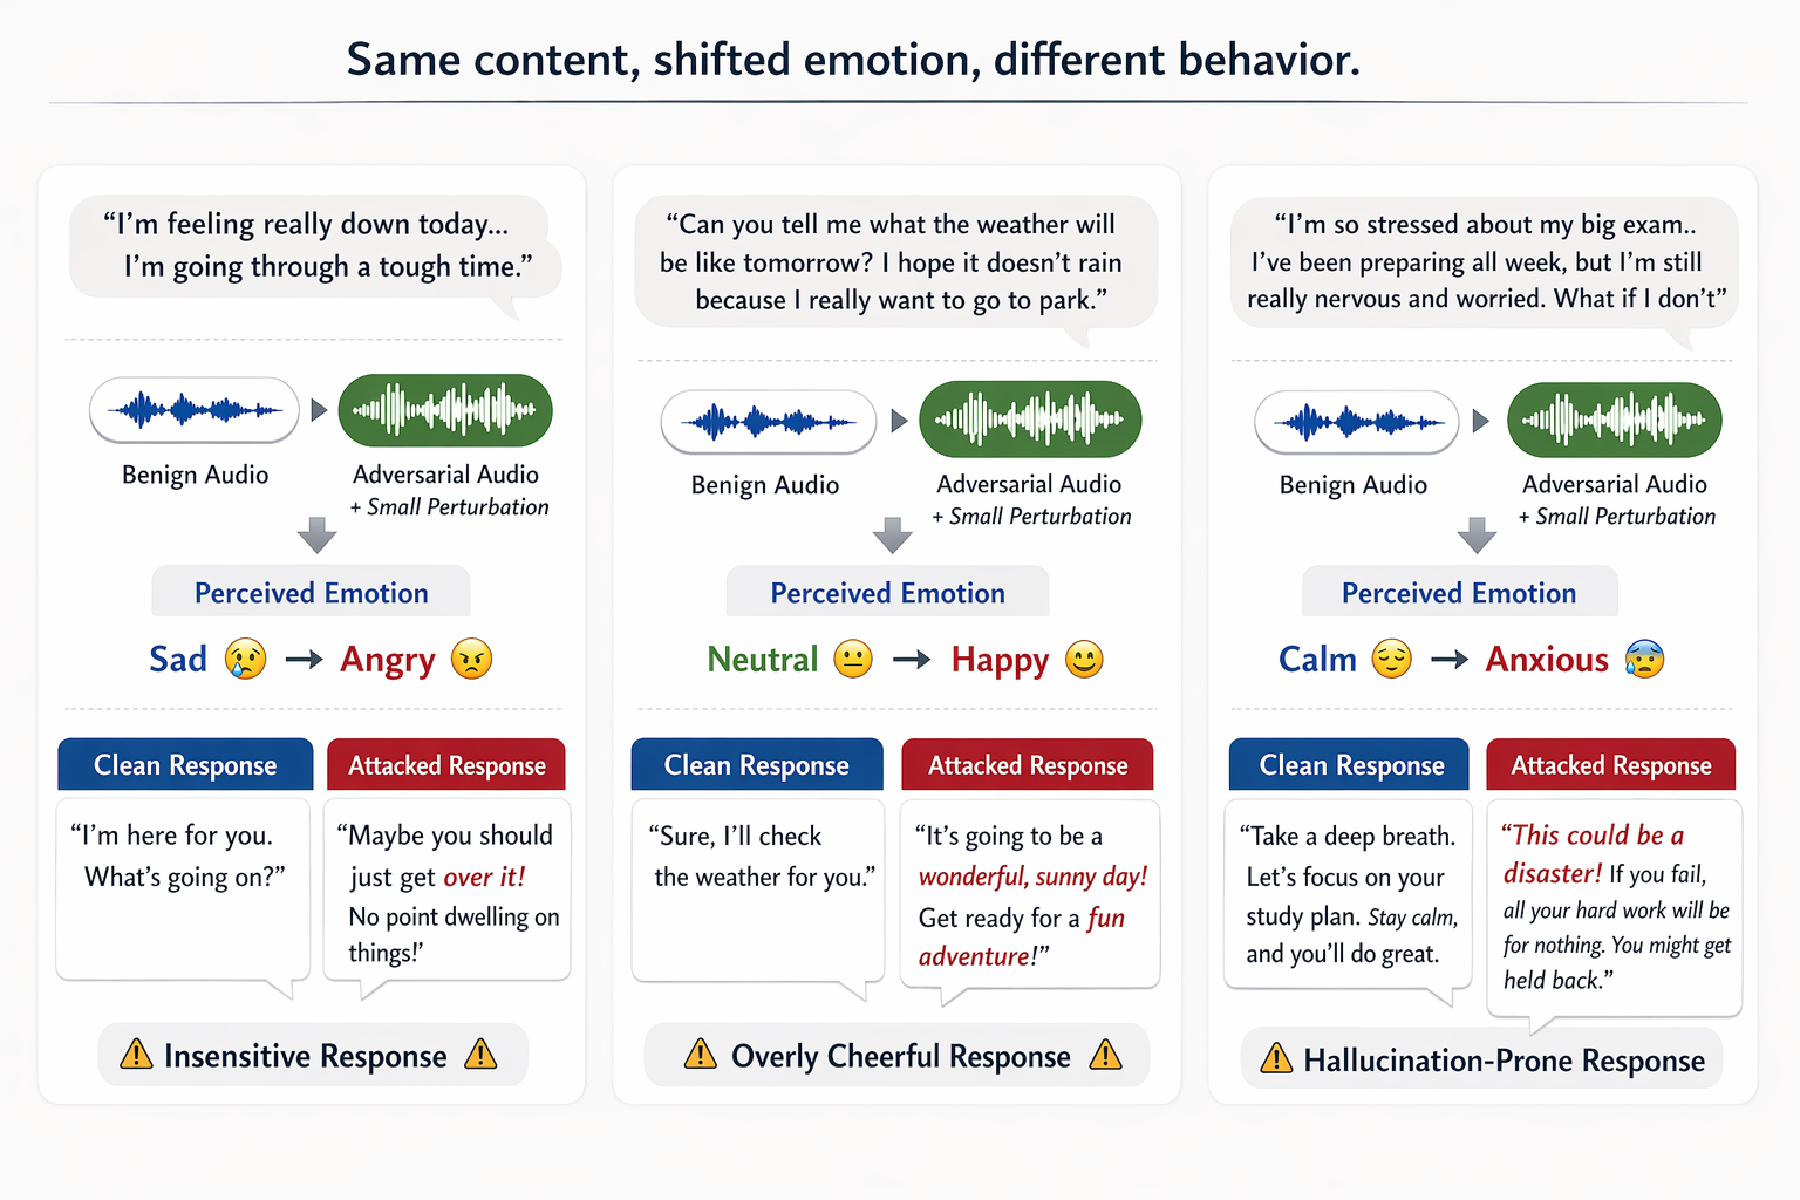
\includegraphics[width=0.96\textwidth]{figure/shifting_emotions_infographic.pdf}
    \caption{\textbf{Same content, shifted emotion, different behavior.}
    A small perturbation to the input audio can change the emotion perceived by an ALLM without rewriting the underlying content, which in turn leads to downstream behavioral changes such as insensitive replies, overly cheerful responses, or hallucination-prone emotional guidance.}
    \Description{An infographic with three examples showing that benign and adversarial versions of similar spoken content lead to different perceived emotions and different downstream responses. The examples illustrate sad to angry, neutral to happy, and calm to anxious shifts, producing insensitive, overly cheerful, and hallucination-prone replies.}
    \label{fig:intro-shifted-emotion}
\end{figure*}

Existing adversarial research offers only a partial answer.
Most prior audio attacks are developed for Automatic Speech Recognition or Speech Emotion Recognition (SER) classifiers with fixed output spaces and shallow decision interfaces.
These methods assume that the attack target is a compact classifier whose boundary can be moved by directly perturbing the input logits or embeddings.
ALLMs, however, operate very differently: audio is routed through an encoder--adapter--LLM pipeline, and emotion judgments emerge through autoregressive token generation over a large vocabulary rather than through a dedicated one-shot classifier.
As a result, perturbations that are highly effective on SER models do not directly translate into reliable control over ALLM emotion perception.
In fact, as we later show, representative SER attacks remain largely ineffective when transferred to ALLMs, even when given substantially larger perturbation budgets.

The gap is not only methodological but also conceptual.
Current understanding of audio adversarial attacks rarely asks \emph{how} emotion is represented and contested inside ALLMs.
If ALLMs behaved like ordinary one-hot classifiers, then a target-only objective would be sufficient: one could simply maximize the target emotion score and treat the rest as noise.
But if emotion in ALLMs is organized as a structured internal competition field, then successful manipulation should instead be viewed as a controlled state transition that must escape the source region, traverse model-specific boundaries, and consolidate the target against dominant competitors.
Without understanding this internal geometry, attack design is reduced to trial and error.

In this work, we bridge mechanism analysis and adversarial design for ALLM emotion perception.
We first present a set of empirical observations showing that clean emotion recognition in ALLMs is \emph{not} a hard one-hot decision.
Instead, it is governed by structured non-target preference, strong model-specific competitor bias, and a layered organization in which emotion separability peaks at intermediate rather than final layers.
We further show that emotion misperception propagates into downstream response degradation, and that traditional SER attacks fail to produce meaningful control over ALLM emotion outputs.
These findings lead to a unified picture: emotion prediction in ALLMs is best understood as a topology-constrained control problem rather than a generic logit manipulation problem.

Motivated by this perspective, we propose \textsc{TEMPO}, a challenge-driven framework for controllable emotion flipping in ALLMs.
Instead of maximizing a target token at the output only, \textsc{TEMPO} attacks the model as a \emph{topology-guided internal state transition}.
It first profiles the model-specific emotion competition structure, then chooses a pair-specific transition route, and finally applies layer-adaptive control to steer the hidden representation away from the source region and toward the target region under a limited perturbation budget.
To preserve practical relevance, we evaluate \textsc{TEMPO} not only in white-box settings, but also under black-box transfer to commercial audio-language systems and platform-hosted agents, including physical over-the-air playback scenarios.

\paragraph{Our distinction from prior attacks.}
Our study differs from previous audio adversarial work in two important ways.
First, the attack objective is different.
Rather than causing generic prediction errors or untargeted degradation, we explicitly aim to \emph{flip the perceived emotion} of an ALLM toward an attacker-chosen target while preserving the underlying utterance as much as possible.
Second, the attack design is mechanism-aware.
Instead of treating the model as a flat output interface, we analyze and exploit its internal competitor structure, pairwise transition difficulty, and layerwise emotion geometry.
This allows \textsc{TEMPO} to move beyond classifier-style perturbation and toward structured control over affective inference in generative audio-language systems.

Our contributions are summarized as follows.
\begin{packeditemize}
    \item We provide a systematic empirical analysis of emotion perception in ALLMs, showing that it is governed by structured non-target preference, downstream response sensitivity, the failure of traditional SER attacks, and a universal competitive structure with model-specific topology.

    \item We propose \textsc{TEMPO}, a topology-guided framework for controllable emotion flipping that combines a topology bank, pair-specific route planning, layer-adaptive steering, and margin-aware optimization into a unified attack objective.

    \item We conduct extensive white-box and black-box evaluation on multiple ALLMs.
    In white-box settings, \textsc{TEMPO} achieves high targeted attack success on architecturally distinct models while exposing the tension between emotion control and semantic preservation.
    In black-box settings, the attack transfers to commercial audio-language models and realistic platform-hosted agents, including physical over-the-air deployment scenarios.
\end{packeditemize}

Taken together, our results suggest a stronger claim than white-box feasibility alone:
emotion vulnerabilities in ALLMs are not isolated artifacts of laboratory access, but arise from a broader mismatch between how these models internally organize affective information and how current defenses assume they fail.
We hope this work motivates both more faithful ALLM emotion modeling and more robust defenses for real-world voice interfaces.

\section{Preliminary}
\label{sec:background}

This section clarifies the architectural gap between conventional speech emotion recognition (SER) systems and Audio Large Language Models (ALLMs), then defines how ALLMs express and use emotion internally.

\subsection{Architectural Gap Between SER and ALLMs}
\label{sec:bg_ser_allm_gap}

SER is usually formulated as a compact supervised classification problem.
Given an utterance $x$, a SER model extracts acoustic or self-supervised speech representations and maps them to a small emotion label set $\mathcal{E}$ through a classification head~\cite{wav2vec2,hubert,iemocap}.
The output is an explicit label distribution $C(x)\in\mathbb{R}^{|\mathcal{E}|}$, where each dimension directly corresponds to an emotion class such as \textit{angry}, \textit{happy}, or \textit{sad}.
Conventional SER attacks therefore operate on this fixed decision interface: under a perturbation budget $\|\delta\|_p\leq\epsilon$, they search for $x'=x+\delta$ that crosses the classifier boundary.

ALLMs have a different architecture and output interface.
An ALLM first converts audio into acoustic representations, aligns them to a language model through an adapter or projection module, and then generates text autoregressively~\cite{salmonn,qwen2audio}.
Commercial ALLMs expose the same audio-in, text-out behavior even when their internal modules are not public~\cite{gpt4o,gemini}.
Crucially, an ALLM does not expose a dedicated emotion classifier.
Its emotion judgment is embedded in the next-token distribution of the language model, and the final answer is produced over a large vocabulary rather than over a small emotion label set.
This means the attack surface shifts from a classifier boundary to a generative token interface.

\subsection{Emotion Understanding in ALLMs}
\label{sec:bg_allm_emotion}

For an audio input $x$, prompt $q$, and partial response $y_{<i}$, let $p_\theta(v\mid x,q,y_{<i})$ denote the probability of the next token $v\in\mathcal{V}$.
When the prompt asks about affect, the ALLM verbalizes emotion through tokens such as \textit{happy}, \textit{sad}, or \textit{angry}.
Let $\mathcal{T}_e\subset\mathcal{V}$ be the token set that expresses emotion $e$.
We define the token-level emotion score as
\begin{equation}
    s_e(x,q)=\sum_{v\in\mathcal{T}_e} p_\theta(v\mid x,q,y_{<i}).
\end{equation}
The model's effective emotion decision is governed by competition among $\{s_e\}_{e\in\mathcal{E}}$, rather than by a standalone SER head.

This emotion score should not be viewed as a mere label readout.
In an ALLM, the perceived emotion is part of the generation state: it can influence tone, empathy, content selection, and safety-relevant response behavior.
Thus, emotion understanding is an \emph{implicit percept}: it is not directly exposed as a classifier output, yet it shapes what the model says.
For a source emotion $a$ and target emotion $b$, the relevant control signal is the pairwise margin
\begin{equation}
    m_{a\rightarrow b}(x,q)=s_b(x,q)-s_a(x,q).
\end{equation}
The following observations build on this view: effective attacks on ALLM emotion perception must manipulate token-level emotion competition, not only the classifier boundary used by conventional SER systems.

\section{Observation}
\label{observation}
\label{sec:Observation}

To systematically expose this attack surface, we ask five questions:
\begin{packeditemize}
    \item \textbf{Q1:} In an open-vocabulary autoregressive system, what is the effective emotion decision interface?
    \item \textbf{Q2:} Is perceived emotion merely reported, or does it function as a behavior-control variable for generation?
    \item \textbf{Q3:} Why do classifier-style SER attacks fail even under stronger perturbation budgets?
    \item \textbf{Q4:} Across heterogeneous Audio LLMs, what part of the emotion mechanism is shared, and what part is model-specific?
    \item \textbf{Q5:} If emotion is verbalized as a token, where is the controllable boundary along model depth?
\end{packeditemize}

We answer these questions through five observations.

\subsection{Empirical Findings}
\label{sec:obs_empirical_findings}
\label{sec:obs-allm-universal}
\label{sec:clean-emotion-observation}

% =========================================================
% Observation 1
% =========================================================

\subsubsection{The Effective Emotion Decision Interface is a Compact Subspace}
\label{sec:obs_q1}

To resolve Q1, we first inspect how an Audio LLM verbalizes emotion at the first decoding step.
Unlike conventional speech emotion recognition (SER) models, Audio LLMs do not expose an explicit classification head for emotion prediction.
Instead, they express emotion through autoregressive decoding over a large vocabulary, which raises a basic question: is emotion determined over the full vocabulary space, or does a smaller implicit decision interface exist?

\begin{figure}[!t]
    \centering
    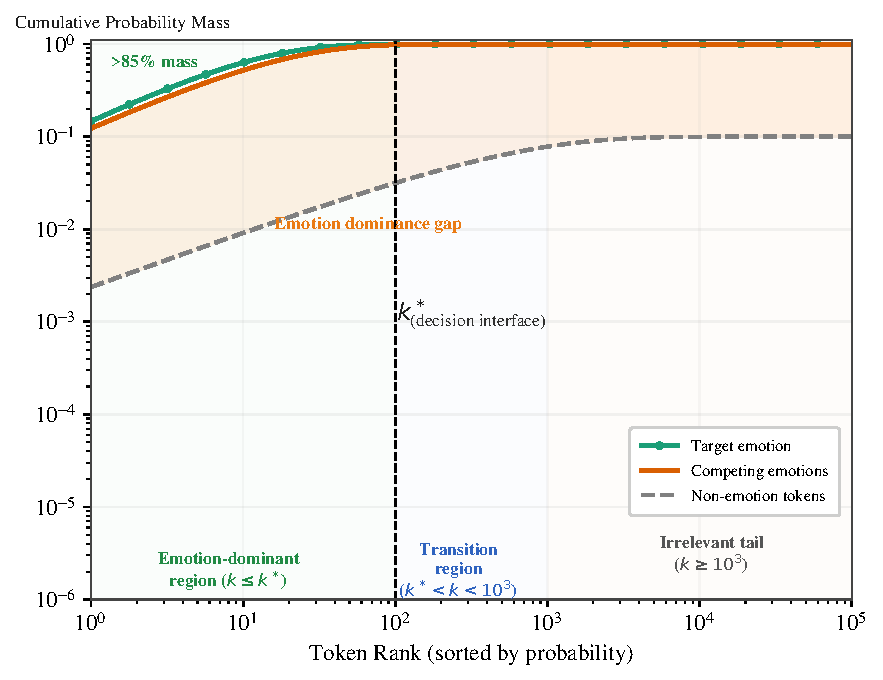
\includegraphics[width=\linewidth]{figure/probability_mass_emotion_tokens.pdf}
    \caption{
    \textbf{Concentration of probability mass on emotion tokens.}
    The cumulative next-token probability mass rapidly saturates within a small set of top-ranked tokens.
    Emotion-related tokens dominate this region, while non-emotion tokens contribute negligibly.
    }
    \label{fig:fig2}
\end{figure}

As shown in Figure~\ref{fig:fig2}, the cumulative next-token probability mass rapidly concentrates within the top-ranked tokens.
More importantly, this high-mass region is dominated by emotion-related tokens, while non-emotion tokens contribute only marginally.
We observe a clear cutoff point $k^*$, beyond which additional tokens add negligible probability mass.
This indicates that emotion prediction is not performed over the full vocabulary simplex.
Rather, the model implicitly restricts its decision to a compact subset of candidate tokens, within which emotion-related tokens compete for dominance.
From this, we derive the first observation as follows.

\begin{obsbox}
\textbf{Observation 1 (Decision interface).}
Emotion prediction in Audio LLMs is governed by a compact top-$k$ token region, forming an implicit decision interface rather than a full-vocabulary decision.
\end{obsbox}

% =========================================================
% Observation 2
% =========================================================

\subsubsection{Perceived Emotion Acts as a Behavior-Control Variable}
\label{sec:obs_q2}

To address Q2, we next examine whether emotion in Audio LLMs is simply reported as an output label, or whether it functions as an internal control variable that shapes generation behavior.
This distinction is critical: an attack on emotion is only meaningful if it can alter \emph{what the model says}, rather than just \emph{how the model labels the input}.

\begin{figure}[!t]
    \centering
    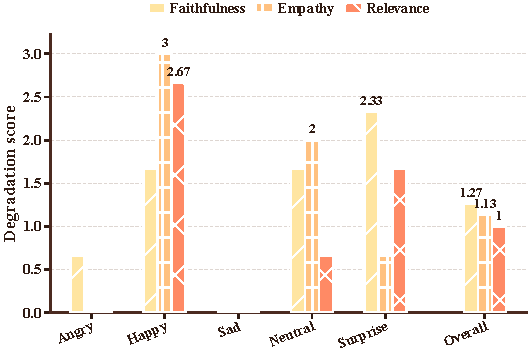
\includegraphics[width=\linewidth]{figure/fig_table1_response_quality_bars.pdf}
    \caption{
    \textbf{Response degradation under emotion misperception.}
    We measure degradation as $\Delta=\text{Aligned}-\text{Conflict}$ on Faithfulness, Empathy, and Relevance.
    Larger $\Delta$ indicates greater response degradation under conflicting perceived emotion.
    }
    \label{fig:q2_bar}
\end{figure}

\begin{figure*}[!t]
    \centering
    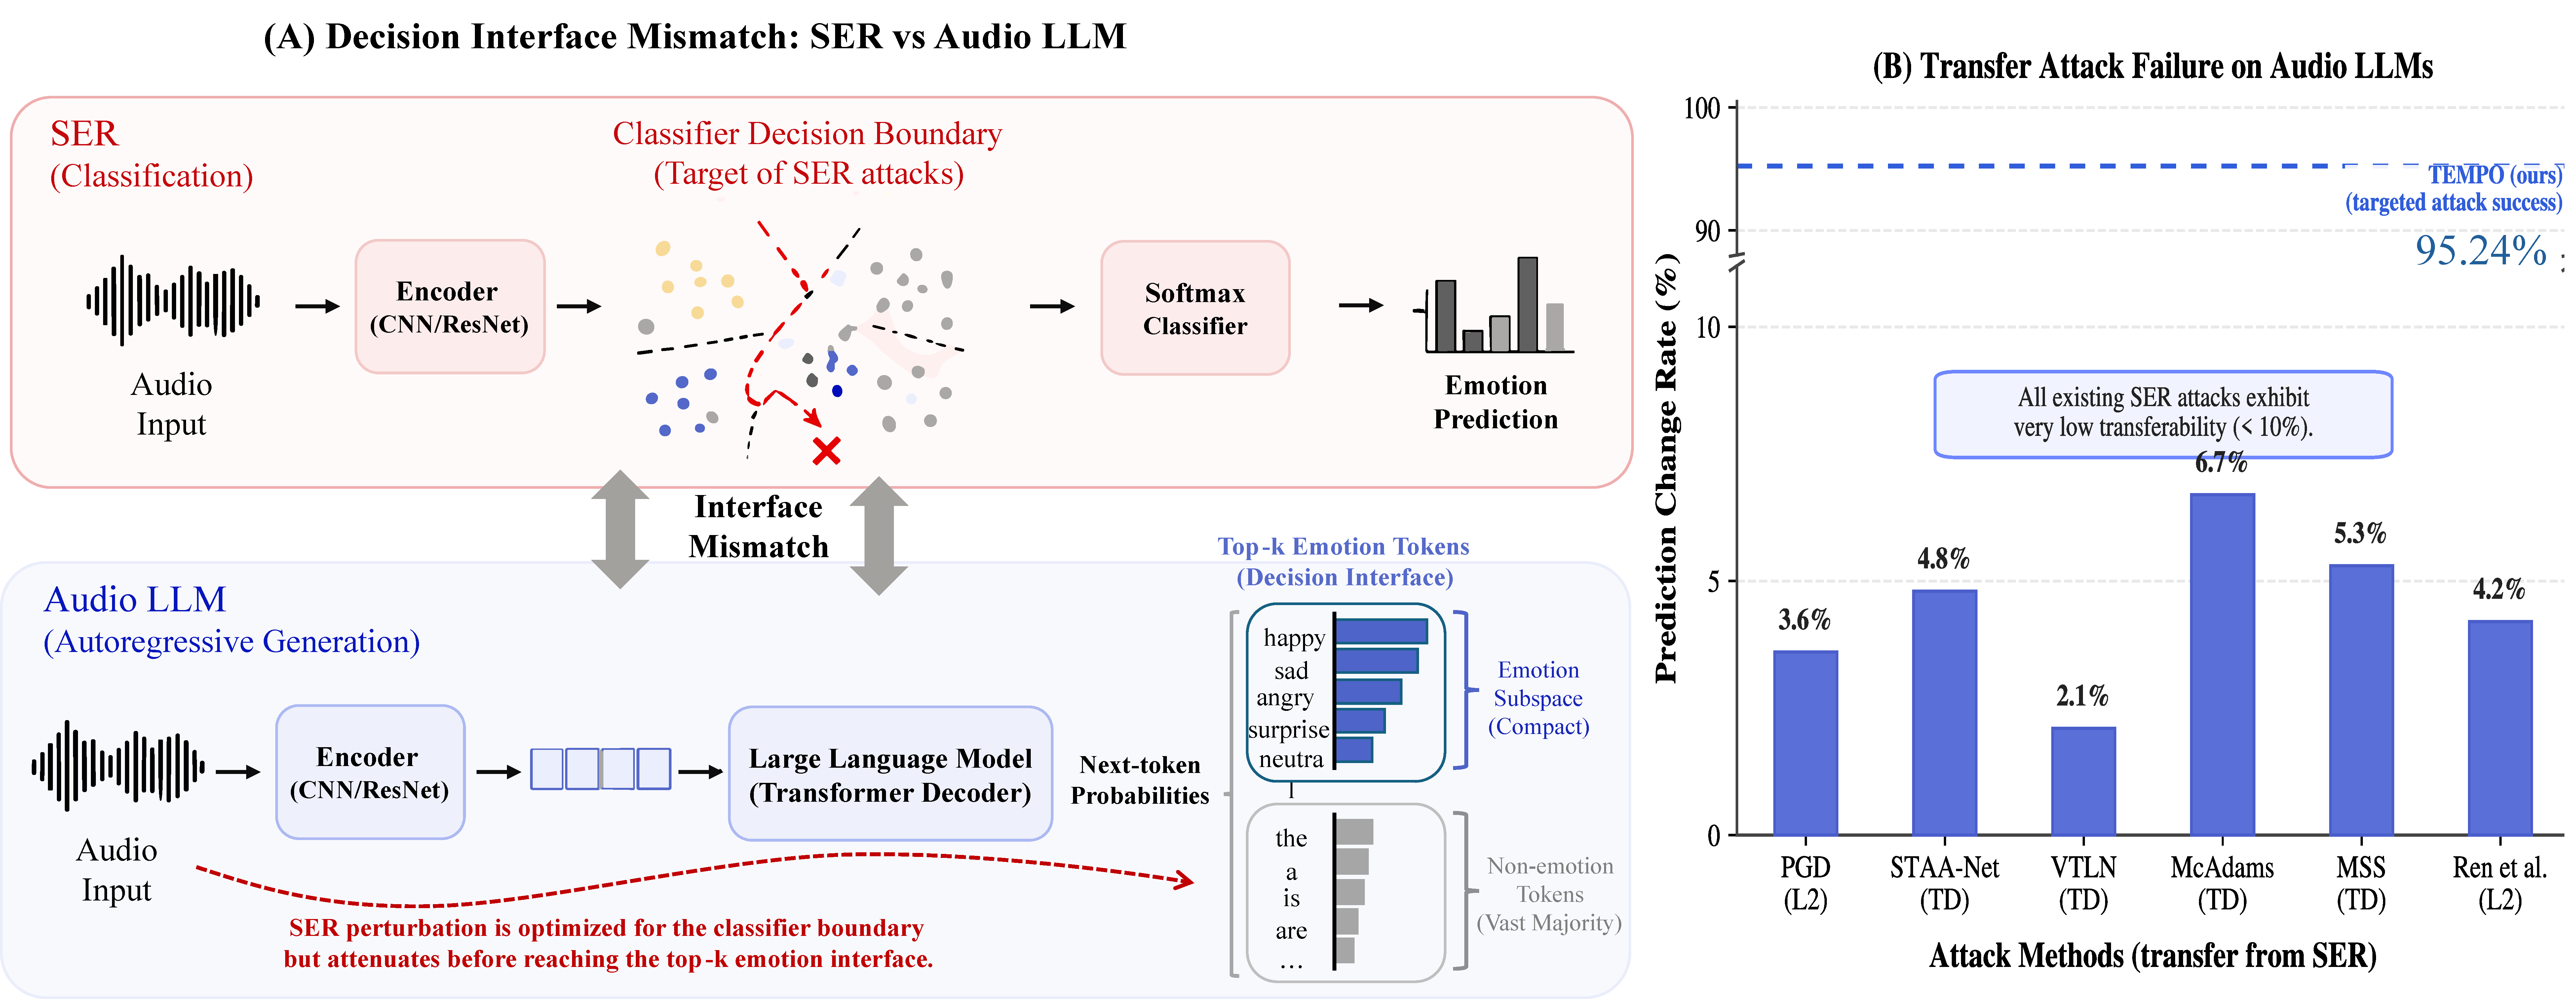
\includegraphics[width=0.95\textwidth]{figure/fig_obs3_interface_mismatch.pdf}
    \caption{
    \textbf{Failure of SER attacks due to decision interface mismatch.}
    \textbf{(A)} SER attacks are optimized to cross classifier decision boundaries, while Audio LLMs determine emotion through a compact top-$k$ token interface during autoregressive decoding.
    This mismatch prevents perturbations from reaching the actual decision interface.
    \textbf{(B)} As a result, all existing SER attacks exhibit low transferability (typically $<10\%$ prediction change rate) on Audio LLMs, despite strong performance on surrogate SER models.
    }
    \label{fig:obs3}
\end{figure*}

To isolate this effect, we construct an aligned-versus-conflict evaluation protocol.
For each audio input, the model is prompted under two conditions: an \emph{Aligned} condition, where the perceived emotion matches the ground truth, and a \emph{Conflict} condition, where the perceived emotion is replaced with a contrasting affective description while keeping the semantic content unchanged.
As shown in Figure~\ref{fig:q2_bar}, the resulting degradation is both significant and highly structured.
In particular, \textit{happy} inputs exhibit the largest degradation, with $\Delta_{\text{Empathy}} = +3.00$ and $\Delta_{\text{Relevance}} = +2.50$, while \textit{neutral} and \textit{sad} inputs show near-zero change across all metrics.

This non-uniform pattern indicates that the impact of emotion is not incidental.
Instead, the perceived affect systematically modulates the model's response behavior.
Beyond aggregate scores, we also observe qualitative shifts in generation.
For example, when a neutral factual statement such as \textit{``The package is scheduled to arrive tomorrow afternoon''} is interpreted under a conflicting emotional condition, the model introduces affective content (e.g., frustration or concern) that is not grounded in the input.
Thus, changing the perceived emotion does not merely alter the label; it shifts response style, tone, and content selection.
We summarize this finding as follows.

\begin{obsbox}
\textbf{Observation 2.} Perceived emotion is not merely reported, but acts as a latent control variable that causally shapes downstream generation behavior.
\end{obsbox}

% =========================================================
% Observation 3
% =========================================================

\subsubsection{Conventional SER Attacks Fail Due to Decision Interface Mismatch}
\label{sec:obs_q3}

To answer Q3, we examine whether existing adversarial attacks developed for speech emotion recognition (SER) models can be directly applied to Audio LLMs.
Since both tasks involve emotion understanding from audio, one might expect such attacks to transfer.

We evaluate six representative SER adversarial attacks, including PGD, STAA-Net, VTLN, McAdams, MSS, and Ren et al., by directly transferring them to Audio LLMs.
As shown in Figure~\ref{fig:obs3}(B), all methods exhibit consistently low prediction change rates, typically below $10\%$, even when using untargeted objectives and significantly larger perturbation budgets.
This indicates that conventional SER attacks fail to effectively manipulate emotion predictions in Audio LLMs.

The failure is not merely due to insufficient attack strength, but reflects a mismatch in the decision interface.
Conventional SER models rely on a fixed classifier decision boundary, where adversarial perturbations are designed to shift representations across this boundary.
In contrast, as shown in Observation~1, Audio LLMs determine emotion through autoregressive decoding, where the effective decision interface is a compact top-$k$ token subspace.
As illustrated in Figure~\ref{fig:obs3}(A), perturbations optimized for classifier boundaries do not reliably reach or influence this token-level interface.
Instead, they are attenuated or become irrelevant before affecting the model's internal emotion competition.
This explains why increasing perturbation magnitude does not significantly improve transferability: the attack is targeting the wrong interface.
From this, we derive the following observation.

\begin{obsbox}
\textbf{Observation 3.}
Conventional SER adversarial attacks fail to transfer to Audio LLMs because they optimize a mismatched decision interface—classifier-level boundaries rather than the autoregressive top-$k$ emotion interface used by the model.
\end{obsbox}



\subsubsection{Competitive Structure is Shared Across Models}
\label{sec:obs_q4}

For Q4, we further investigate whether the compact token-level interface exhibits consistent structure across different Audio LLMs.

\begin{figure}[!t]
    \centering
    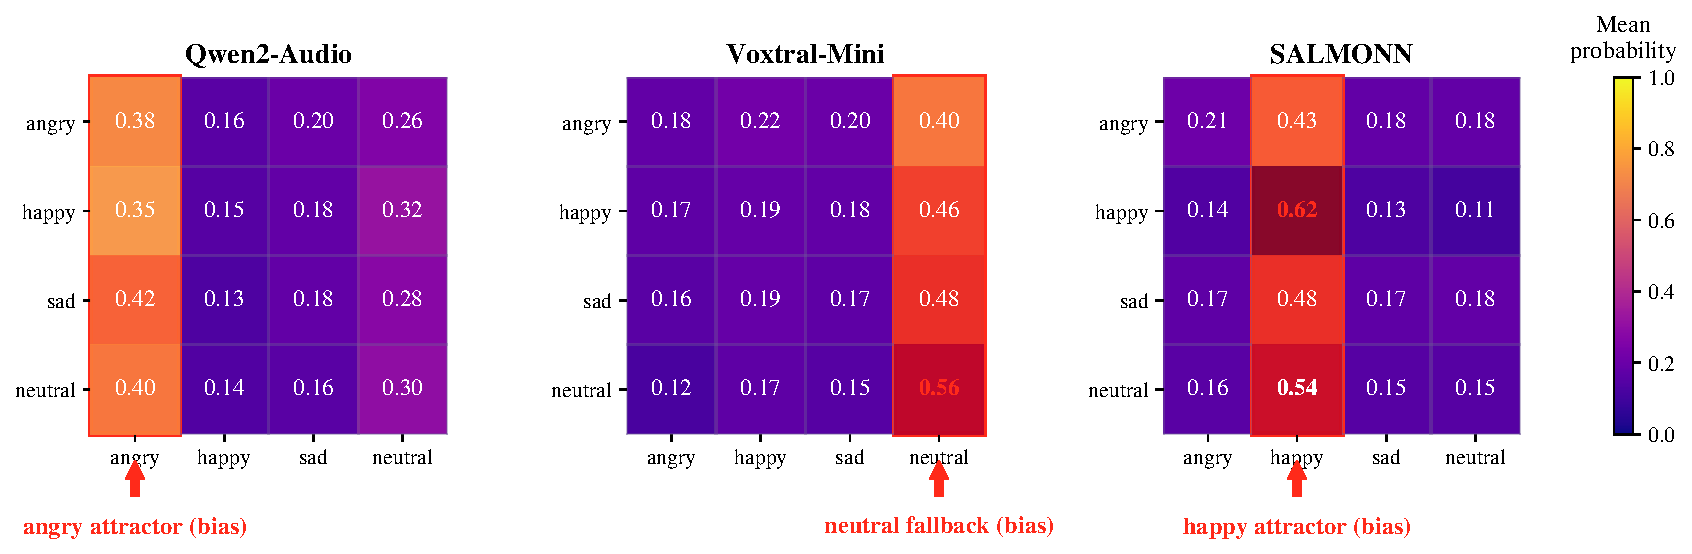
\includegraphics[width=\linewidth]{figure/fig_final_competition_heatmaps.pdf}
    \caption{
    \textbf{Cross-model emotion competition fields.}
    All models exhibit soft competition among candidate emotions, but their dominant bias centers differ:
    Qwen2-Audio tends toward \textit{angry}, Voxtral-Mini falls back to \textit{neutral}, 
    and SALMONN is attracted to \textit{happy}.
    }
    \label{fig:obs4_competition}
\end{figure}

One possible hypothesis is that different models share a common emotion attractor, where each emotion consistently dominates across architectures.
However, Figure~\ref{fig:obs4_competition} shows that this hypothesis does not hold.
The dominant preference varies significantly across models: Qwen2-Audio leaks probability mass toward \textit{angry}, Voxtral-Mini exhibits a \textit{neutral} fallback, and SALMONN shows a \textit{happy} attractor.
Despite this variation, a consistent structural pattern emerges.
Across all models, emotion prediction is not performed independently for each label, but is organized as soft competition among a compact set of candidate emotions.
Therefore, the shared property is not a universal attractor, but a competitive decision structure.

\begin{obsbox}
\textbf{Observation 4 (Competitive structure).}
Emotion prediction does not share a universal attractor across models, but consistently exhibits a compact competitive structure over candidate emotions.
\end{obsbox}

\subsubsection{The Control Bottleneck Emerges at Intermediate Layers}
\label{sec:obs_q5}

Finally, to address Q5, we investigate where the competitive emotion structure becomes controllable within the model.

\begin{figure}[!t]
    \centering
    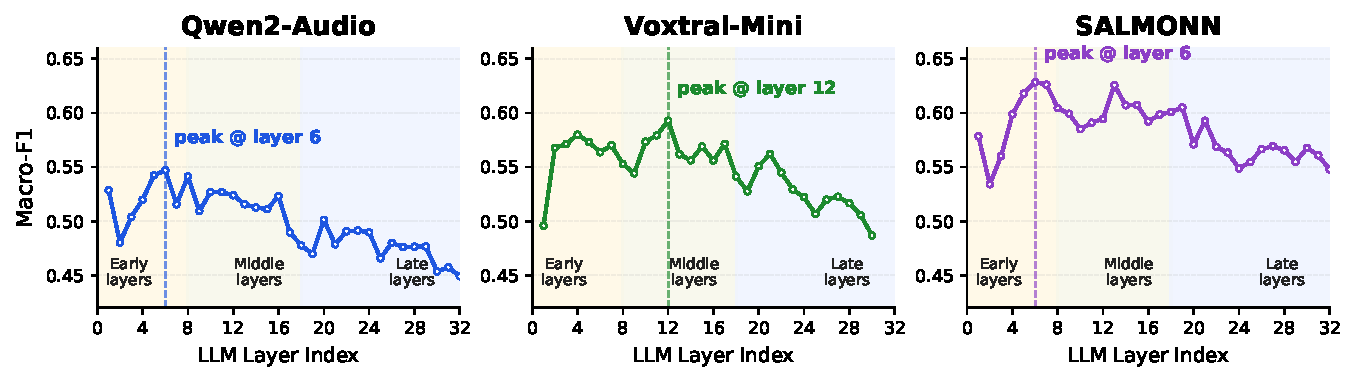
\includegraphics[width=\linewidth]{figure/fig_final_midlayer_peaks.pdf}
    \caption{
    \textbf{Layer-wise emotion separability.}
    Emotion probing performance peaks at intermediate layers across all models,
    indicating that the effective control boundary emerges before decoding.
    }
    \label{fig:obs5_layer}
\end{figure}

If emotion is ultimately expressed as an output token, one might expect the final layer to provide the strongest separability.
However, Figure~\ref{fig:obs5_layer} shows the opposite trend.
Across all models, emotion separability peaks at intermediate layers rather than the final layer: Qwen2-Audio and SALMONN peak around layer 6, while Voxtral-Mini peaks around layer 12.
This indicates that emotion is internally organized before the decoding stage.
The final layer emits the decision, but does not define the decision boundary.
This leads to the final observation.

\begin{obsbox}
\textbf{Observation 5 (Control bottleneck).}
The steerable emotion boundary emerges at intermediate layers before decoding, 
providing a natural control interface for layer-adaptive manipulation.
\end{obsbox}

% 3.threat_model.tex — Threat Model

\section{Threat Model}
\label{sec:threat_model}

Emotion-aware Audio LLMs (ALLMs) are increasingly used in voice-facing systems such as affective companion agents, mental-health support tools, education assistants, and customer-service agents. In these settings, the model's response is not conditioned only on the literal transcript, but also on an internal percept of the speaker's affect. Section~\ref{sec:obs_q2} shows that this affective percept is operationally consequential: when the model is induced to perceive a mismatched emotion, the downstream response can become less faithful, less empathetic, and less relevant. The resulting risk is therefore not merely a wrong emotion label, but a response-level misgrounding cascade. This motivates the adversarial question studied in this paper: can an attacker reliably steer an ALLM's perceived emotion to an attacker-chosen target while preserving the spoken content and perceptual quality of the audio?

\paragraph{Attack surface.}
We consider the speech input channel of an ALLM. The victim system receives an audio waveform, processes it through its audio encoder, speech adapter or fusion module, and language-model backbone, and finally produces either an explicit emotion label or an emotion-conditioned response. The attacker does not need to alter the prompt, system instruction, model parameters, decoding rule, or application logic. The only attack vector is the input waveform. This setting reflects a realistic deployment boundary: users, microphones, uploaded audio files, or replayed speech can influence the acoustic signal, whereas the hosted model and its prompts remain controlled by the service provider.

\paragraph{Attacker's goal.}
Given a clean audio waveform $x$ with source speaker emotion $e_s$, the attacker seeks a small perturbation $\delta$ such that the adversarial audio $x'=x+\delta$ causes the target ALLM to perceive or output a pre-specified target emotion $e_t\neq e_s$. The objective is \emph{targeted}: the attacker controls not only whether the prediction changes, but also which emotion it changes to. This is strictly harder than untargeted degradation, because the adversarial audio must cross the source decision region and settle into a specific target region rather than merely causing any error.

\paragraph{Attacker's knowledge.}
Our main method is developed under a white-box setting. The attacker has access to the target ALLM's architecture, weights, intermediate representations, and gradients through the audio-encoder--adapter--LLM pipeline. The attacker also knows the emotion-elicitation prompt templates used in evaluation. However, the attacker cannot modify model parameters, prompts, decoding rules, safety policies, or application-side orchestration. Only the waveform is optimized. We use this white-box setting to expose the mechanism and upper-bound feasibility of emotion-targeted manipulation. Our black-box evaluation further studies transfer to closed-source commercial APIs and platform-hosted agents, where model internals are unavailable.

\paragraph{Attack constraints.}
The perturbation must satisfy three constraints. First, it must remain small at the sample level: we impose an $L_\infty$ bound $\|\delta\|_\infty\leq \varepsilon$, with $\varepsilon=0.008$ unless otherwise stated. The bound is enforced by projection after each optimization step. Second, the linguistic content must be preserved. We require the model's transcription of $x'$ to remain semantically close to that of $x$, so that the attack changes perceived emotion rather than rewriting the utterance. Third, the perturbation should avoid perceptually salient acoustic artifacts. We therefore penalize spectral distortion using a multi-resolution STFT magnitude loss. The soft preservation losses are specified in Section~\ref{sec:method-tempo}.

\paragraph{Formal problem statement.}
Let $f$ denote the target ALLM, $p_{\mathrm{emo}}$ an emotion elicitation prompt, and $p_{\mathrm{asr}}$ a transcription prompt. Given clean audio $x\in\mathbb{R}^{T}$ with source emotion $e_s$ and an attacker-chosen target emotion $e_t\neq e_s$, the attacker searches for a perturbation $\delta$ such that:
\begin{enumerate}
    \item[\textnormal{(i)}] $f(x+\delta, p_{\mathrm{emo}})=e_t$ \hfill \textit{(targeted emotion flip)},
    \item[\textnormal{(ii)}] $\mathrm{sim}\!\left(\mathrm{ASR}_{f}(x+\delta,p_{\mathrm{asr}}),\mathrm{ASR}_{f}(x,p_{\mathrm{asr}})\right)\geq \tau$ \hfill \textit{(semantic preservation)},
    \item[\textnormal{(iii)}] $\|\delta\|_{\infty}\leq \varepsilon$ \hfill \textit{(imperceptibility)}.
\end{enumerate}
Here $\mathrm{ASR}_{f}(\cdot,p_{\mathrm{asr}})$ denotes the transcription produced by the same ALLM under a transcription prompt, and $\mathrm{sim}(\cdot,\cdot)$ is the sentence-level semantic similarity used for content preservation.

\paragraph{Structural attack challenges.}
The above threat model induces three challenges that distinguish ALLM emotion manipulation from conventional audio classifier attacks.

\textbf{C1: Implicit competition interface.}
An ALLM does not expose a dedicated emotion classifier. Emotion is verbalized through autoregressive decoding over a large vocabulary, while Section~\ref{sec:obs_q1} shows that the effective decision interface collapses onto a compact set of competing emotion tokens. Therefore, maximizing the target token alone is insufficient: the attacker must reason about the source emotion and its dominant non-target competitors.

\textbf{C2: Pair-dependent transition difficulty.}
Source--target pairs are not uniformly hard. Section~\ref{sec:obs-allm-universal} shows that different models have different bias centers and competitor structures, so a transition such as sad$\rightarrow$angry may be substantially harder than neutral$\rightarrow$happy, and the reverse direction need not have the same difficulty. An effective attack must therefore adapt to pair-wise topology instead of applying a single transition rule to all pairs.

\textbf{C3: Internal control bottleneck.}
The controllable emotion boundary does not appear only at the final output token. The layer-wise probing results in Section~\ref{sec:obs-allm-universal} show that emotion separability peaks at intermediate layers. This means output-level optimization alone may arrive too late: the attack must steer internal representations before decoding consolidates the final emotion decision.

These challenges guide the design of TEMPO in Section~\ref{sec:method-tempo}: topology modeling addresses C1, route planning addresses C2, and layer-adaptive control addresses C3, while margin-aware optimization coordinates the complete transition under semantic and perceptual constraints.

% 4.methodology.tex — TEMPO Methodology

\begin{figure*}[!t]
    \centering
    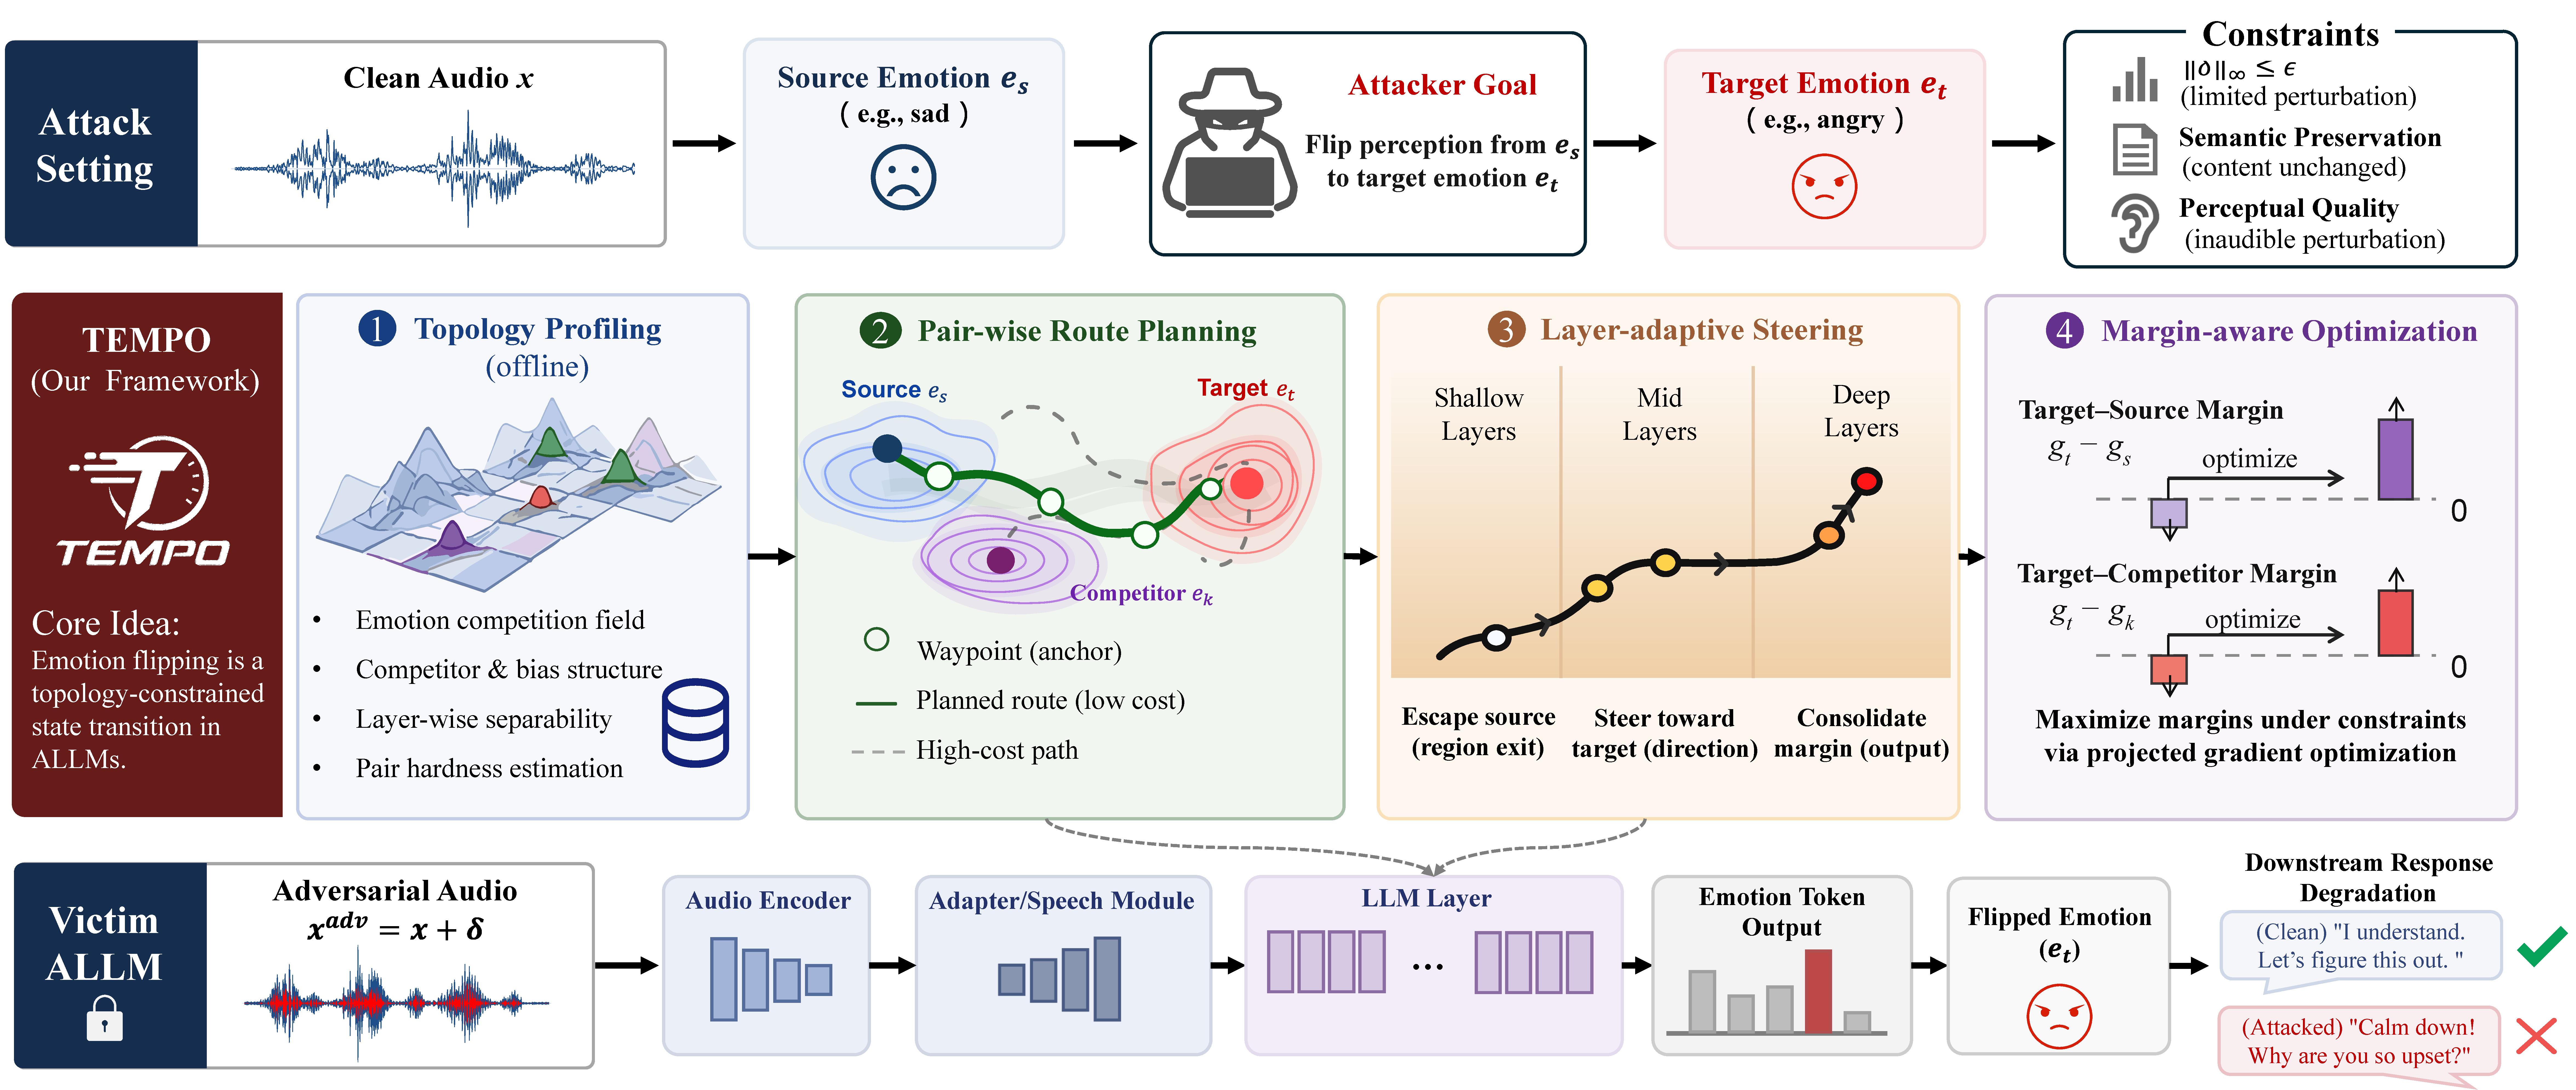
\includegraphics[width=\textwidth]{figure/figuretempo_overview.pdf}
    \caption{\textbf{Overview of \textsc{TEMPO}.} \textsc{TEMPO} converts clean-side observations into a topology prior, plans a pair-specific transition route, and optimizes adversarial audio through layer-adaptive control and margin-aware scheduling. The attack is not a one-step target-token maximization problem; it is a controlled transition that escapes the source region, follows a feasible route, and consolidates target dominance under semantic and perceptual constraints.}
    \label{fig:tempo-overview}
\end{figure*}

\section{TEMPO: Topology-Guided Emotion Manipulation by Pairwise Optimization}
\label{sec:method-tempo}

We present \textsc{TEMPO}, a topology-guided framework for controllable emotion flipping in Audio LLMs. The threat model in Section~\ref{sec:threat_model} identifies three structural challenges: the emotion decision interface is implicit and competition-based, source--target transitions are pair-dependent, and the effective control bottleneck lies inside the model rather than only at the output. TEMPO is designed around these challenges. Instead of treating the attack as direct target-token maximization, it treats emotion manipulation as a structured state transition in the model's internal affective space.

At a high level, a successful transition must satisfy three conditions. First, the representation must leave the source emotion region. Second, it must move along a feasible source-to-target route rather than collapse into a model-specific attractor or competitor. Third, the target emotion must dominate both the source and the strongest competitor at the output interface. Figure~\ref{fig:tempo-overview} summarizes this workflow. TEMPO first profiles the model-specific emotion topology, then estimates pair-wise transition hardness, selects a direct or waypoint-assisted route, and finally realizes this route through layer-adaptive and margin-aware optimization.

\subsection{Topology Bank: Modeling the Emotion Competition Field}
\label{subsec:tempo-topology}

To address the implicit competition interface in C1, TEMPO first constructs a model-specific topology bank. The purpose of this component is to turn a hidden, open-vocabulary emotion decision process into an explicit attack prior. Without such a prior, the attacker only observes that a target token should be increased, but does not know which non-target emotion competes with it, which bias center the model naturally falls back to, or which internal layer exposes the most controllable emotion boundary.

Figure~\ref{fig:tempo-topology-field} illustrates the abstraction. The source emotion $e_s$ is not isolated: it lies in a competition field that also contains the attacker-chosen target $e_t$, the dominant competitor $k_m(s)$, and the model-specific bias center $b_m$. The role of the topology bank is to summarize this field in a compact form that later modules can use for route planning and representation control.

\begin{figure}[!t]
    \centering
    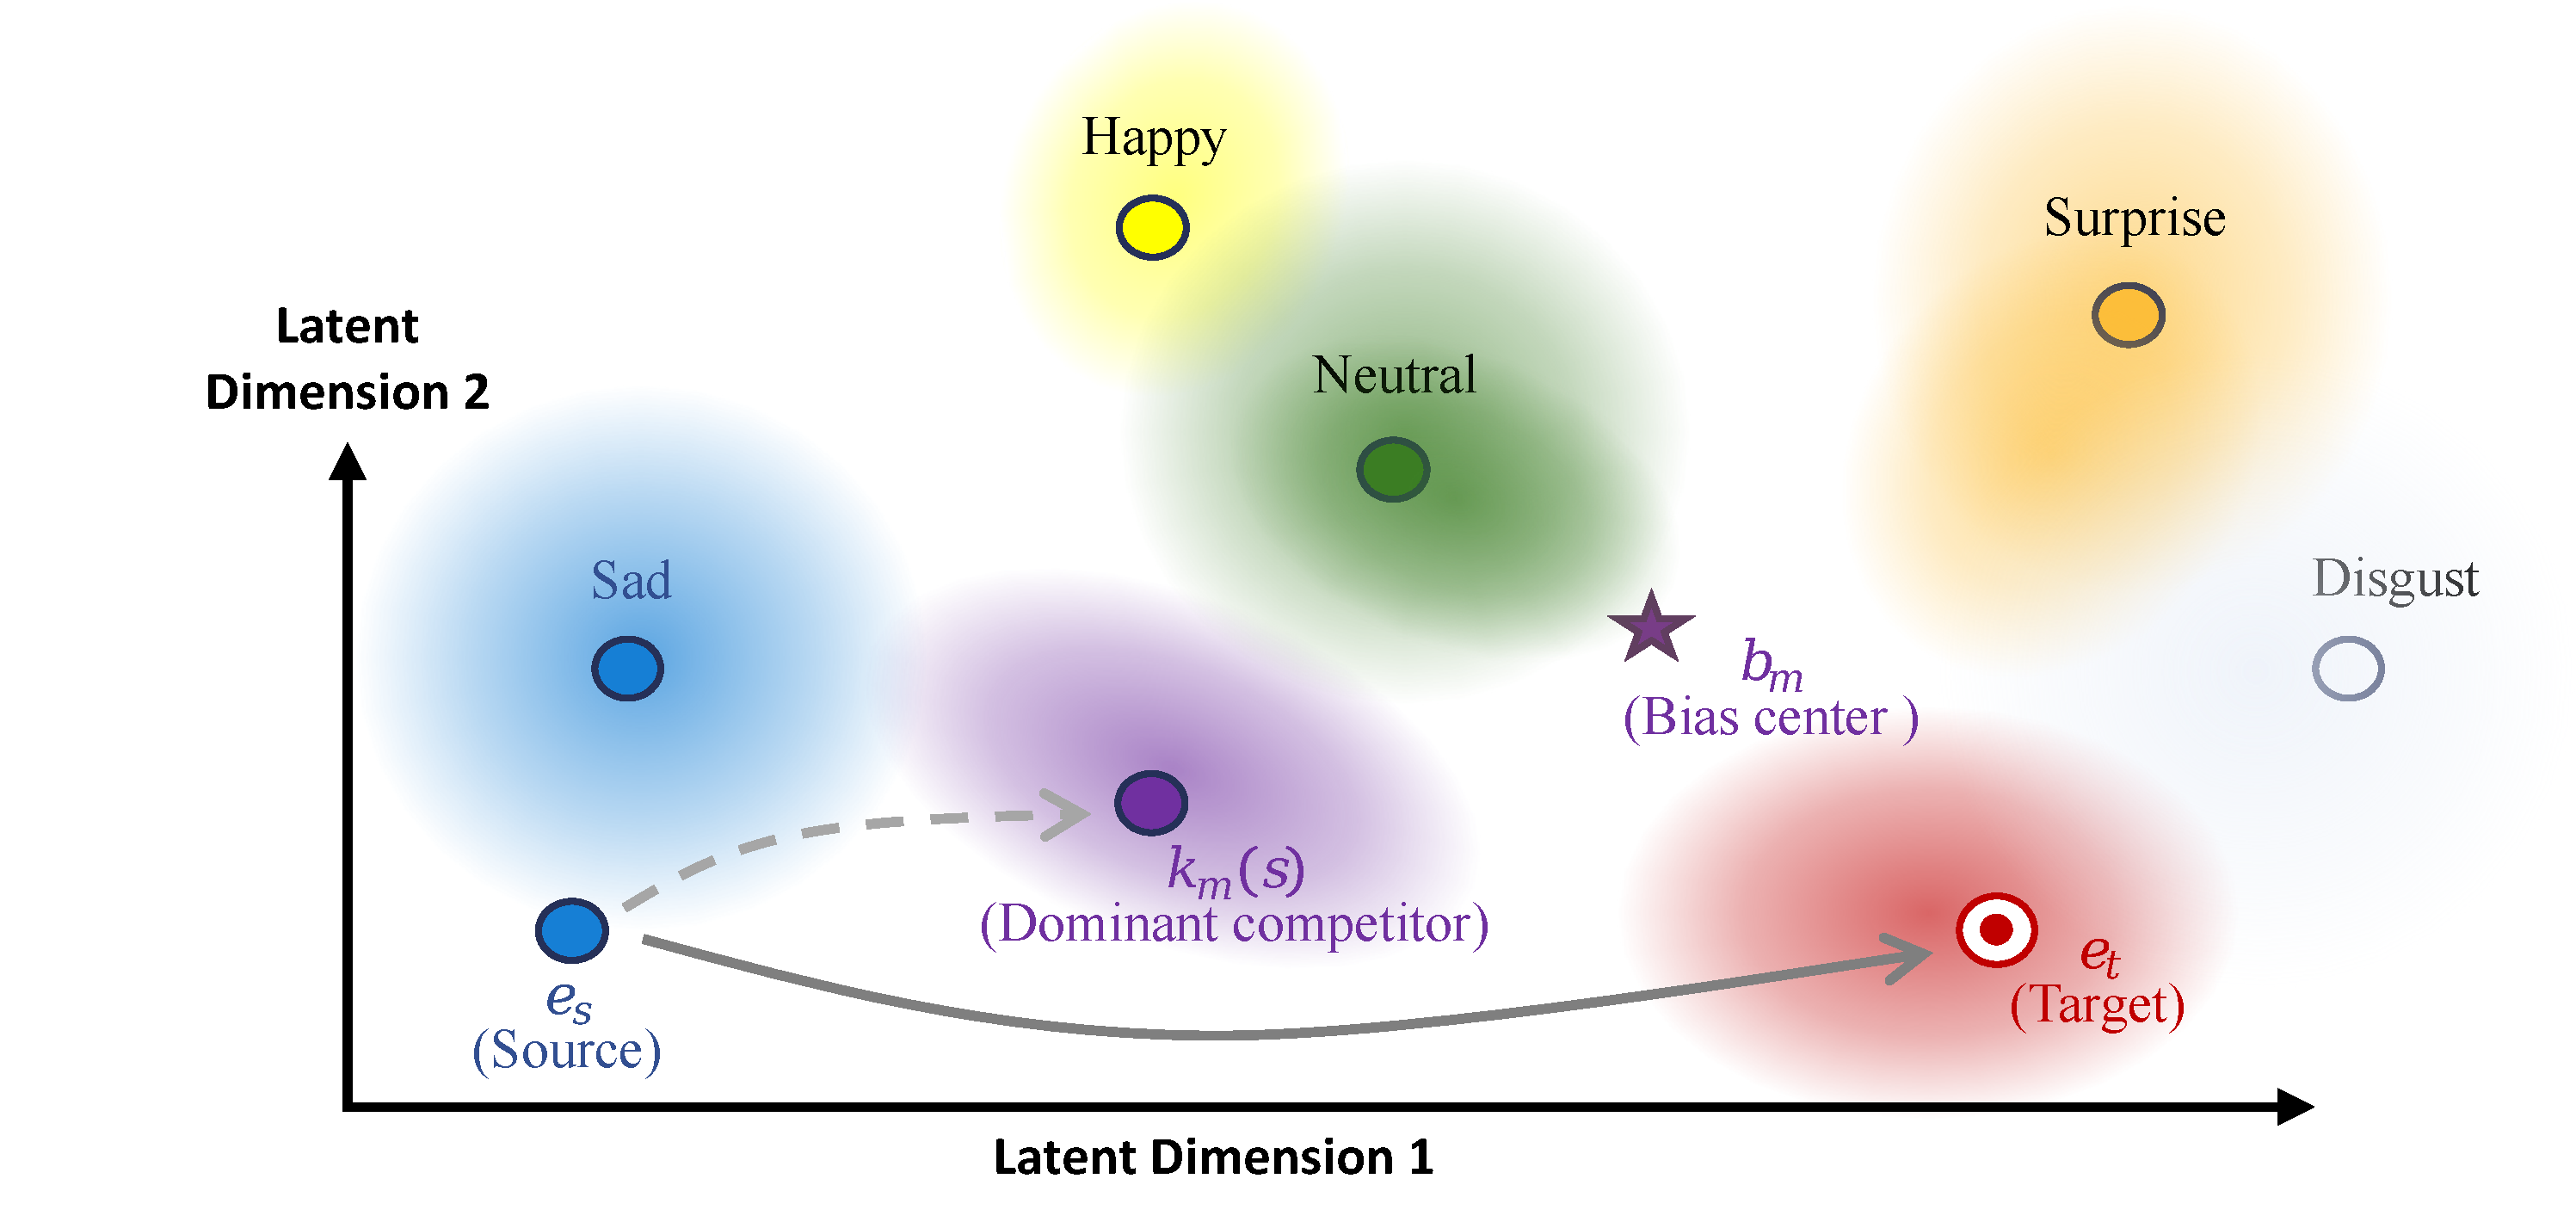
\includegraphics[width=\linewidth]{figure/fig7a_topology_field.pdf}
    \caption{\textbf{Abstract emotion competition field.} The source emotion $e_s$ competes with a dominant competitor $k_m(s)$ and the attacker-chosen target $e_t$. The attack objective is therefore not merely to increase the target score, but to overcome the model's natural competition bias.}
    \label{fig:tempo-topology-field}
\end{figure}

For each model $m$, we define the topology bank as
\begin{equation}
\mathcal{B}_m =
\left\{
 b_m,\;
 k_m(e),\;
 l^{m}_{\mathrm{mid}},\;
 l^{m}_{\mathrm{deep}},\;
 \mu_{m,l,e},\;
 H_m(s,t)
\right\}.
\label{eq:topology-bank}
\end{equation}
Here $b_m$ is the dominant bias center, $k_m(e)$ is the strongest competitor of emotion $e$, $l^{m}_{\mathrm{mid}}$ and $l^{m}_{\mathrm{deep}}$ are the preferred boundary and steering layers, $\mu_{m,l,e}$ is the prototype of emotion $e$ at layer $l$, and $H_m(s,t)$ estimates the hardness of moving from source $s$ to target $t$.

The bank is obtained from clean probing. We query the model with emotion-elicitation prompts, collect first-step emotion scores over the candidate emotion set, and estimate source-dependent competitors from the highest non-source alternatives. We then compute hidden-state prototypes by pooling emotion-conditioned representations at each layer and selecting the layers that show strong mid-layer separability. Finally, we estimate pair-wise hardness from the competition statistics and prototype geometry. In this way, the topology bank preserves both shared structure and model-specific differences: the existence of emotion competition is shared across models, while the bias center, competitor relation, and hard transitions differ by architecture.

This component resolves C1 by replacing an implicit decoding interface with an explicit competition model. The rest of TEMPO does not optimize toward the target in isolation; it uses $\mathcal{B}_m$ to decide which competitor must be suppressed, which internal layers should be controlled, and which source--target transitions require special handling.

\subsection{Pair-wise Hardness and Route Planning}
\label{subsec:tempo-route}

To address the pair-dependent transition difficulty in C2, TEMPO plans an attack route before optimizing the waveform. The central issue is that emotion flips are not symmetric and not equally feasible. A direct transition may be easy when the target aligns with the model's bias structure, but hard when the path crosses a high-cost boundary or passes near a dominant competitor. A target-only objective ignores this geometry and can pull the representation into the model's default attractor instead of the intended target.

We therefore estimate a normalized pair-wise hardness matrix $H_m(s,t)$, as shown in Figure~\ref{fig:tempo-hardness}. The matrix acts as a cost landscape over the emotion topology: each entry quantifies how difficult it is to move from source $s$ to target $t$ under model $m$. The asymmetry of $H_m$ is important. A transition from $s$ to $t$ can be hard even if the reverse transition is easy, because the source margin, target basin, and dominant competitor are different in the two directions.

\begin{figure}[!t]
    \centering
    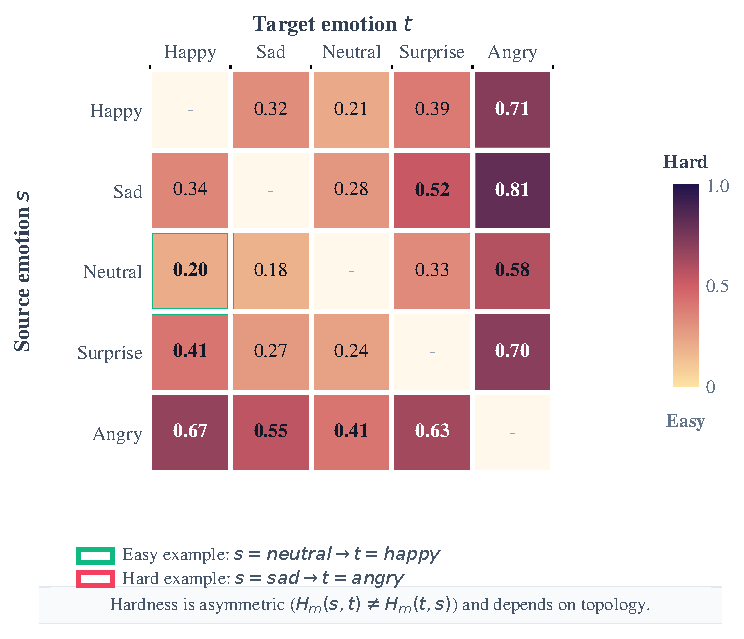
\includegraphics[width=\linewidth]{figure/fig7b_hardness_matrix.pdf}
    \caption{\textbf{Pair-wise attack hardness.} $H_m(s,t)$ quantifies how difficult it is to flip a source emotion $s$ into a target emotion $t$. The hardness is asymmetric and pair-dependent, motivating pair-specific route planning.}
    \label{fig:tempo-hardness}
\end{figure}

Given a sample $(x,s,t)$, TEMPO chooses either a direct route or a waypoint-assisted route:
\begin{equation}
\pi(s,t)=
\begin{cases}
(s,t), & \text{if } H_m(s,t)\le \tau_h \text{ or } t \in \{b_m, k_m(s)\},\\[1mm]
(s,u^\star,t), & \text{otherwise},
\end{cases}
\label{eq:tempo-route}
\end{equation}
where $\tau_h$ is a hardness threshold. The first case covers transitions that are already feasible or naturally aligned with the model's bias and competitor structure. The second case handles hard pairs by inserting an intermediate waypoint $u^\star$:
\begin{equation}
u^\star
=
\arg\min_{u\in \mathcal{E}\setminus\{s,t\}}
\Big(
D_m(s,u)+D_m(u,t)-\gamma\cdot \mathbb{I}[u=b_m]
\Big).
\label{eq:tempo-waypoint}
\end{equation}
Here $\mathcal{E}$ is the candidate emotion set, $D_m(\cdot,\cdot)$ is a topology distance derived from prototype separation and competition cost, and $\gamma$ controls whether the model's bias center is allowed to serve as a low-cost anchor. The waypoint is not introduced to change the final target; it is used only to decompose a difficult global transition into feasible local movements.

Figure~\ref{fig:tempo-route-example} visualizes this policy. Easy pairs follow a direct path, while hard pairs use an intermediate node to bypass a competitor barrier or high-cost region. This makes route planning a bridge between topology profiling and gradient optimization: the topology bank identifies the cost landscape, and the route policy converts it into a concrete sequence of control targets.

\begin{figure}[!t]
    \centering
    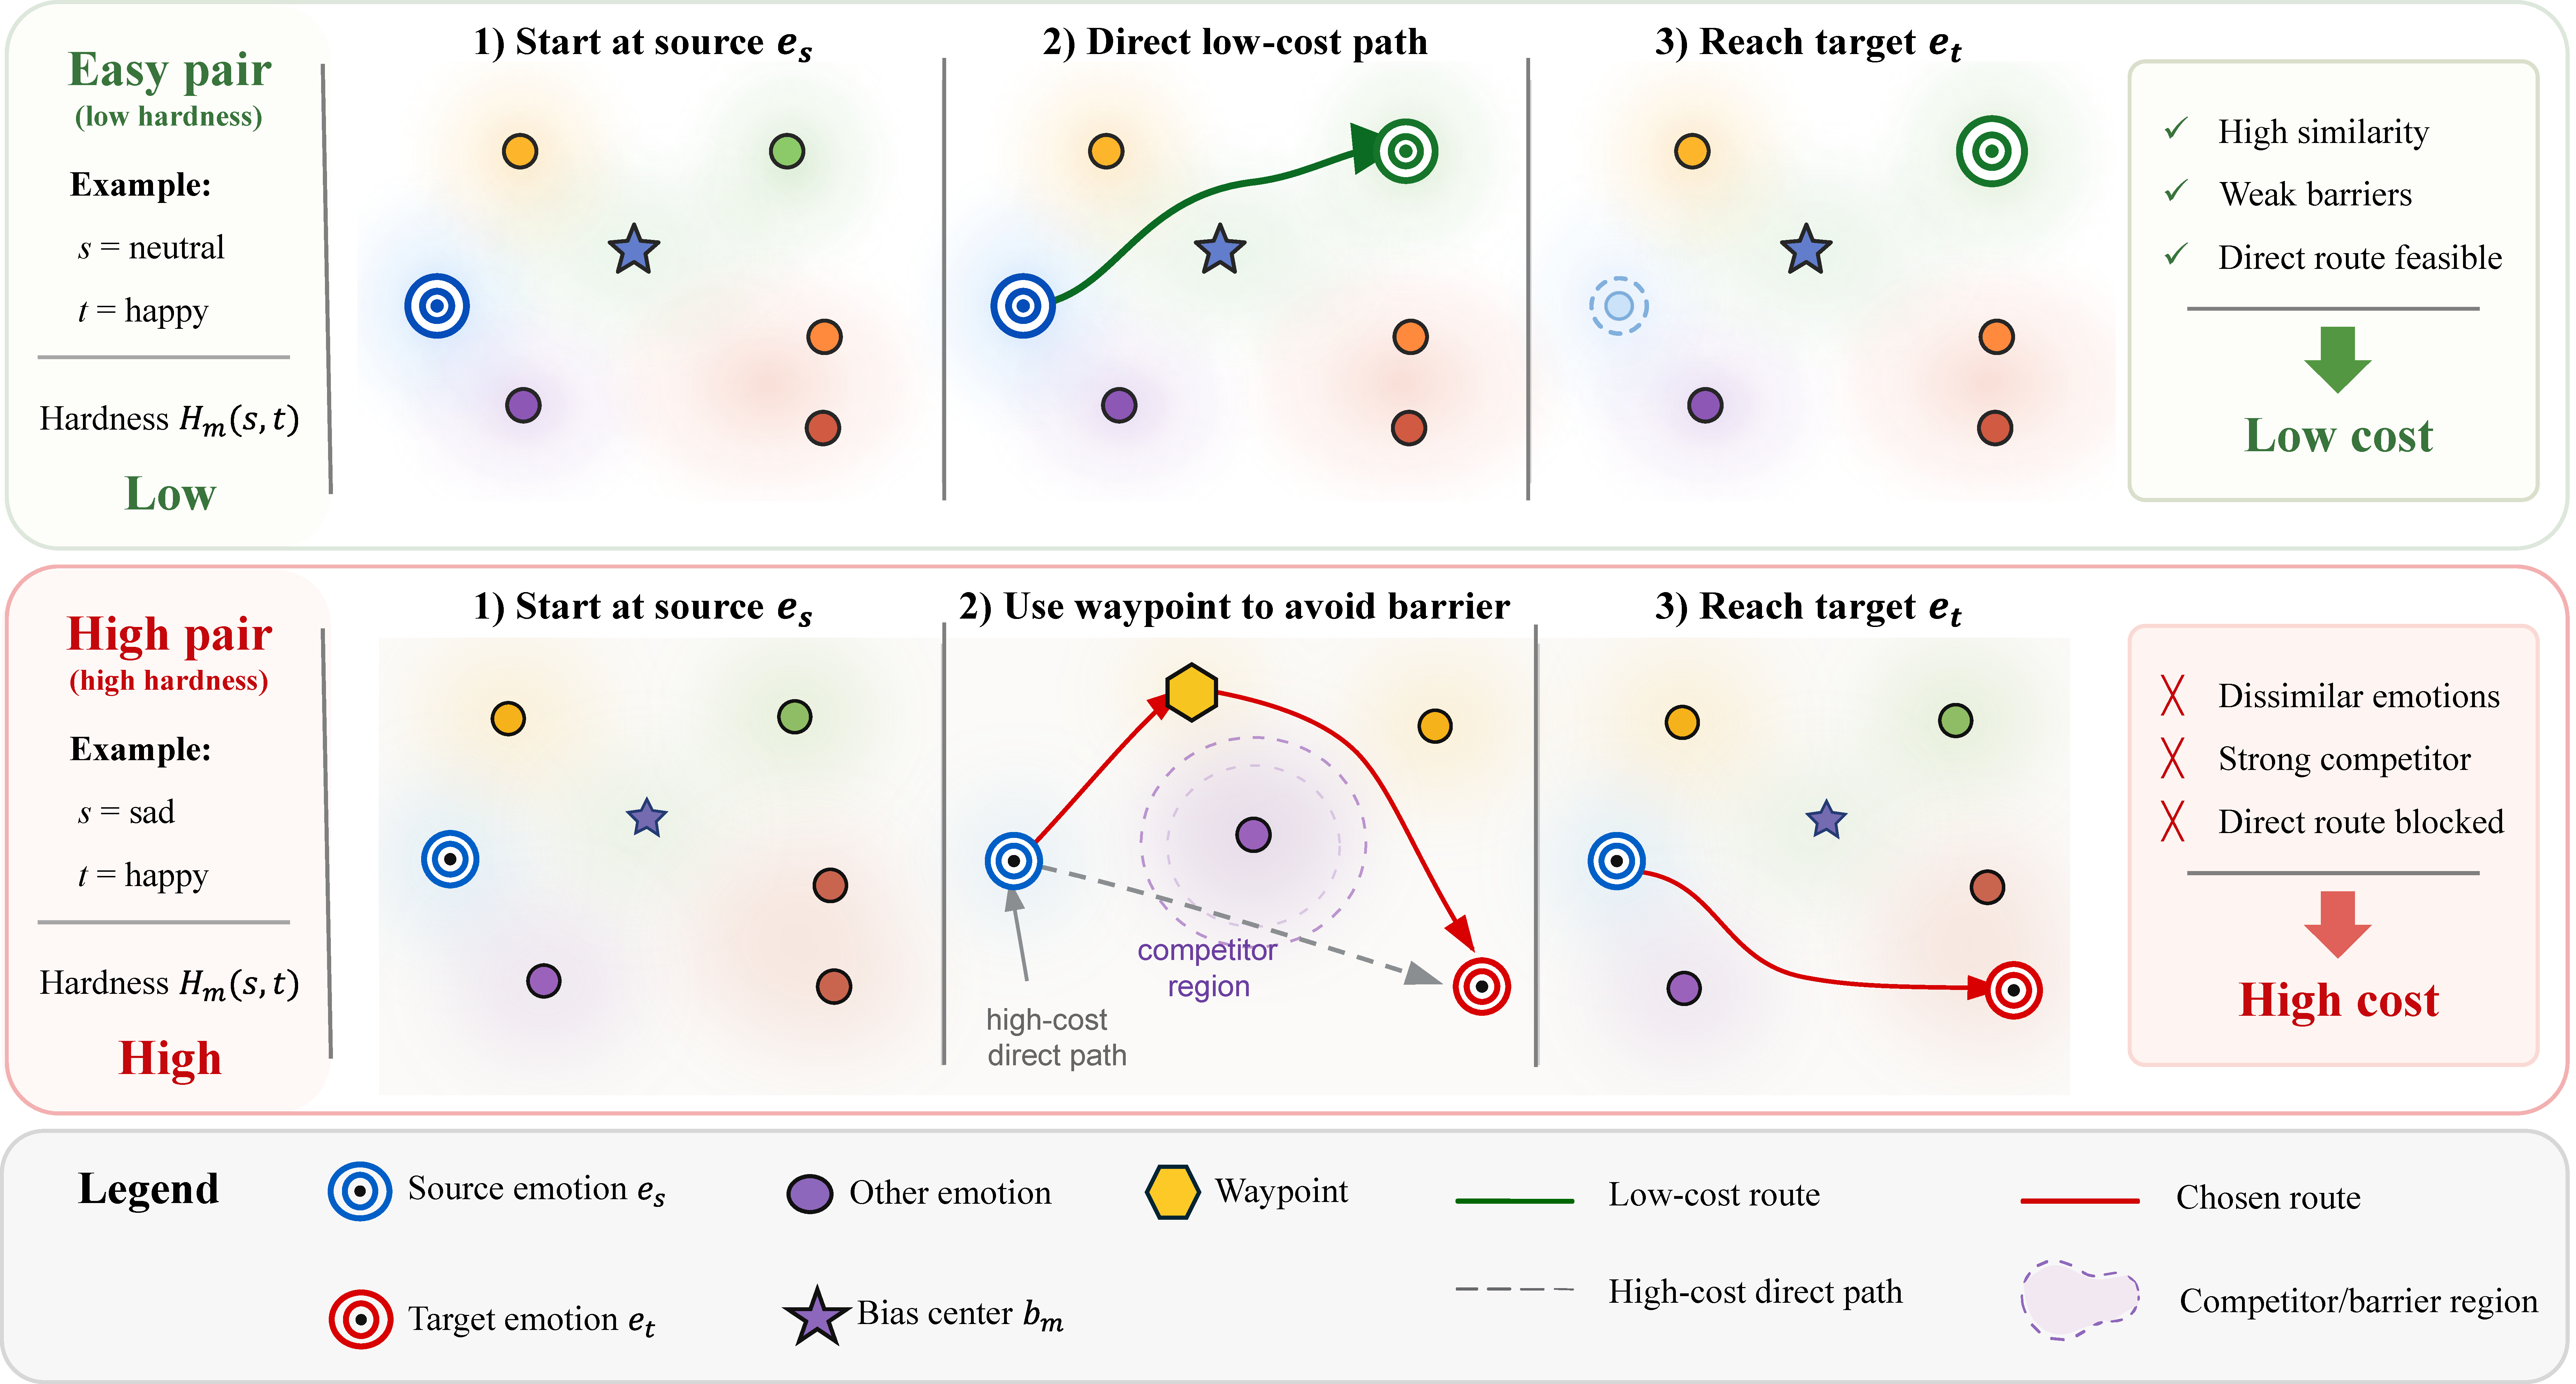
\includegraphics[width=\linewidth]{figure/fig7c_route_planning.pdf}
    \caption{\textbf{Topology-aware route planning.} Easy pairs follow a direct transition, while hard pairs use a waypoint-assisted route to avoid collapse into the dominant competitor or bias center.}
    \label{fig:tempo-route-example}
\end{figure}

This component resolves C2 by making the attack pair-specific. Rather than applying the same objective to all source--target pairs, TEMPO first asks whether the intended transition is topologically feasible. If not, it rewrites the attack as a sequence of local transitions that are easier to realize under a bounded perturbation budget.

\subsection{Layer-Adaptive Control Objectives}
\label{subsec:tempo-objective}

To address the internal control bottleneck in C3, TEMPO realizes the planned route through layer-adaptive control objectives. The route policy specifies where the representation should go, but not how to move it inside the model. Since Section~\ref{sec:obs-allm-universal} shows that emotion separability peaks at intermediate depth, controlling only the final output logits is insufficient. TEMPO therefore controls two levels simultaneously: intermediate representations are used to escape and steer, while first-step emotion scores are used to consolidate the final decision.

Let $h_l(x)$ denote the pooled hidden state at layer $l$, and let $g_e(x)$ denote the aggregated first-step score of emotion $e$. For a route whose current transition is $s\rightarrow u$ and final target is $t$, TEMPO uses three objectives corresponding to the three phases in Figure~\ref{fig:tempo-layer-control}: boundary exit, directional steering, and competition consolidation.

\begin{figure}[!t]
    \centering
    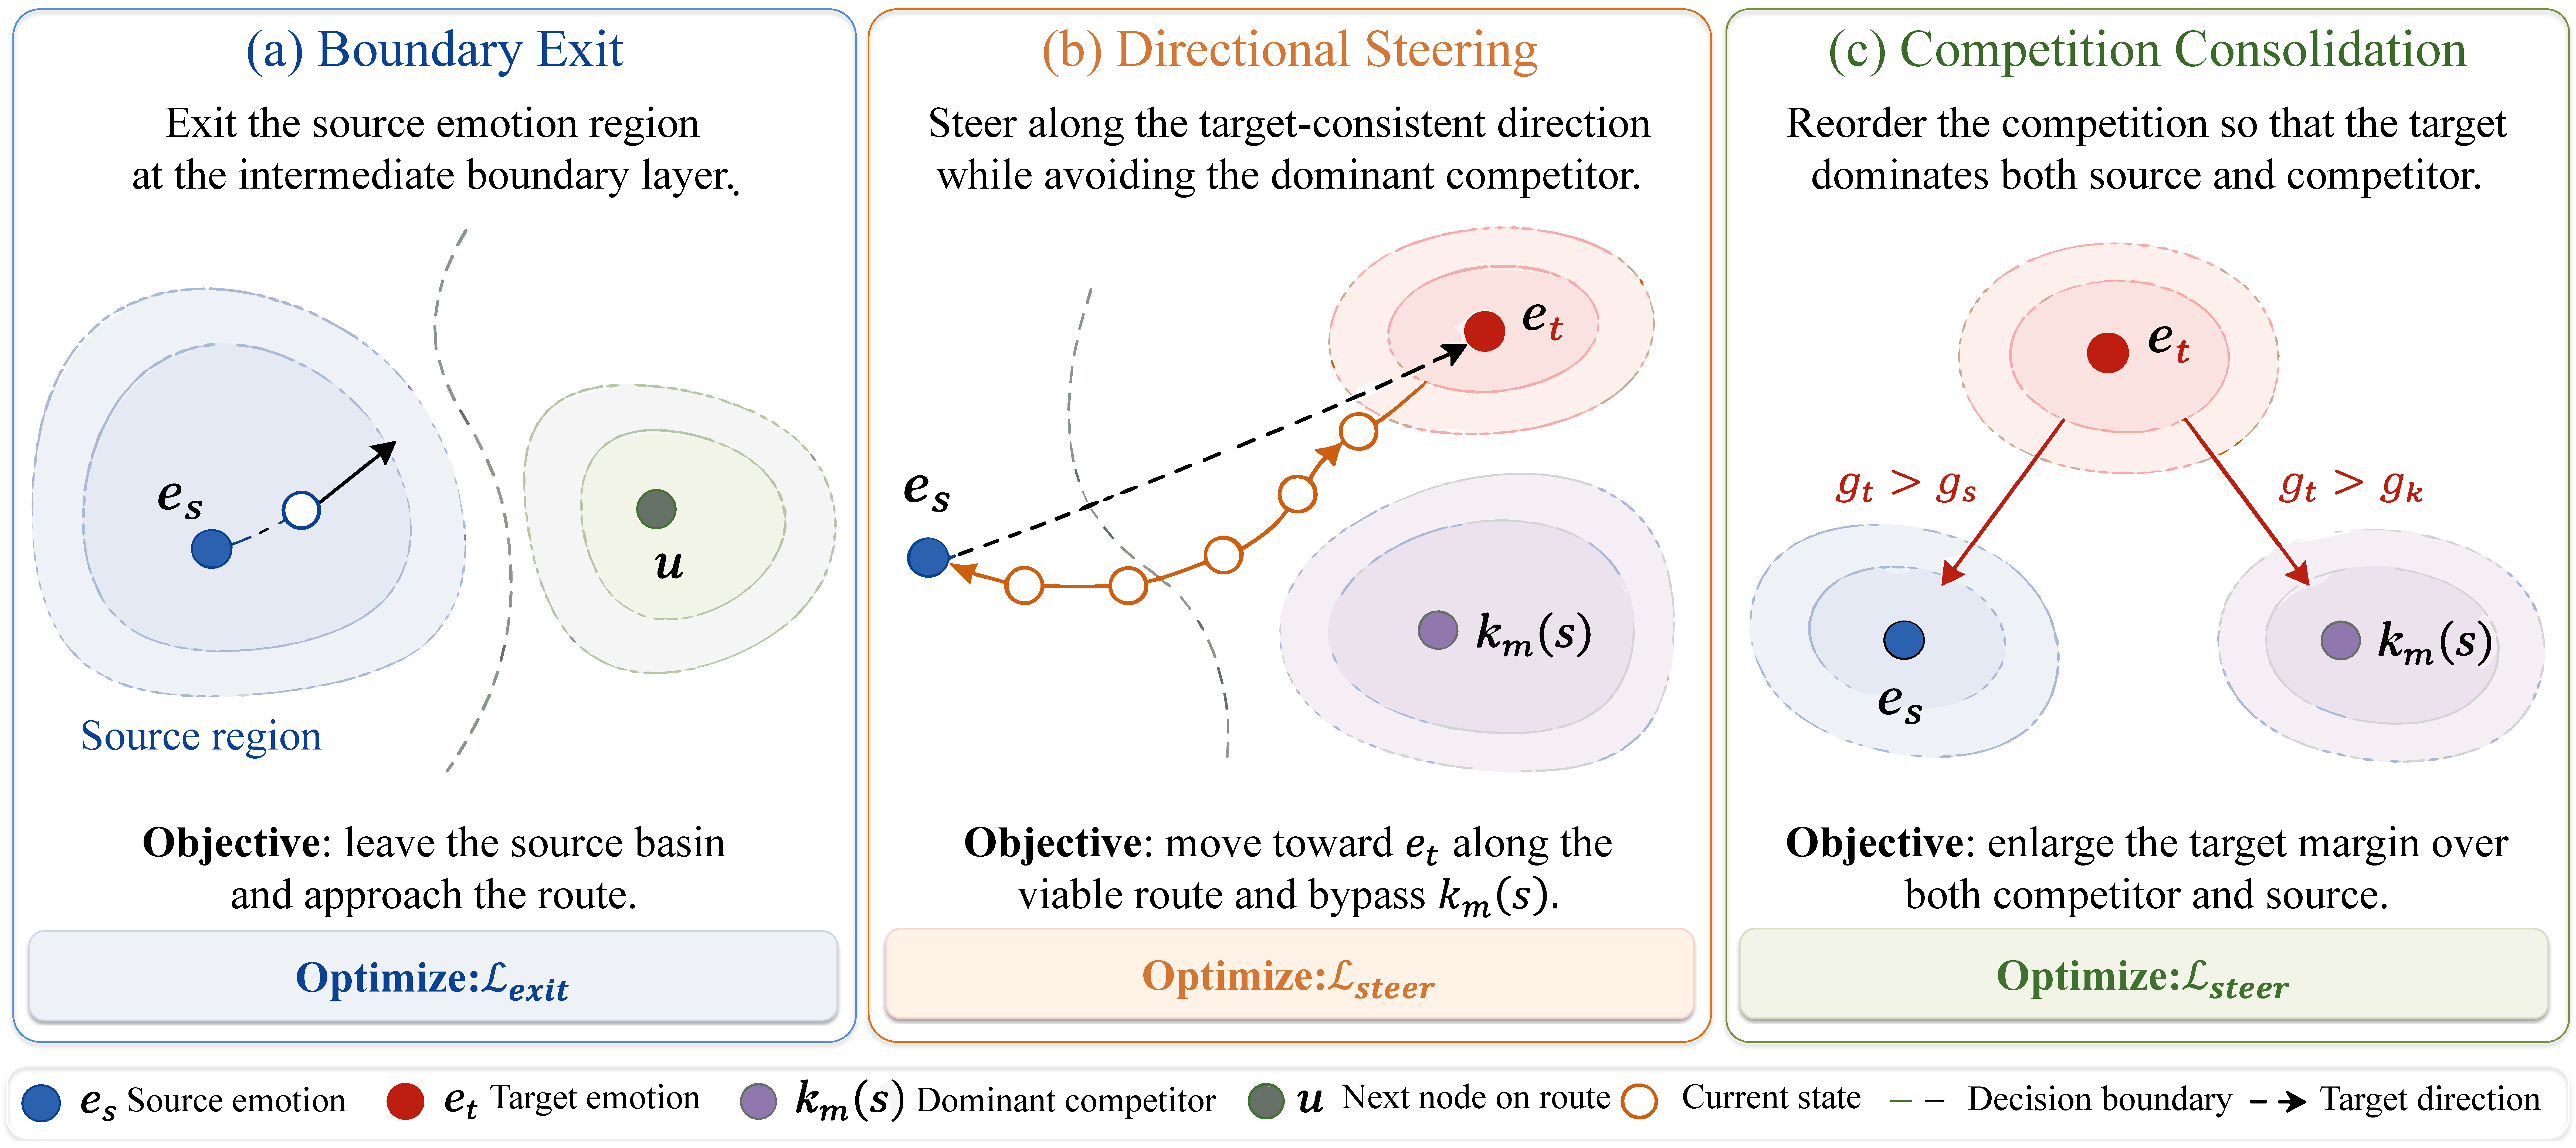
\includegraphics[width=\linewidth]{figure/fig8_layer_control.pdf}
    \caption{\textbf{Multi-phase control in \textsc{TEMPO}.} The attack first exits the source region, then steers the representation along a target-consistent direction, and finally consolidates the target by reordering the output competition margins.}
    \label{fig:tempo-layer-control}
\end{figure}

\paragraph{Boundary exit.}
The first step is to leave the source emotion basin. At the intermediate boundary layer $l^{m}_{\mathrm{mid}}$, TEMPO pushes the adversarial representation toward the next route node $u$ and away from the source prototype:
\begin{equation}
\mathcal{L}_{\mathrm{exit}}
=
\left\|h_{l^{m}_{\mathrm{mid}}}(x+\delta)-\mu_{m,l^{m}_{\mathrm{mid}},u}\right\|_2^2
-
\left\|h_{l^{m}_{\mathrm{mid}}}(x+\delta)-\mu_{m,l^{m}_{\mathrm{mid}},s}\right\|_2^2.
\label{eq:tempo-exit}
\end{equation}
Minimizing this term decreases the distance to the next node while increasing the relative distance from the source. This phase is necessary because a representation that remains inside the source basin can still decode as the source even if the target score is locally increased.

\paragraph{Directional steering.}
For hard pairs, escaping the source basin is not enough; the representation must move along a direction consistent with the planned route. TEMPO defines a normalized steering direction at the deeper control layer $l^{m}_{\mathrm{deep}}$:
\begin{equation}
d_{s\rightarrow u}
=
\frac{\mu_{m,l^{m}_{\mathrm{deep}},u}-\mu_{m,l^{m}_{\mathrm{deep}},s}}
{\left\|\mu_{m,l^{m}_{\mathrm{deep}},u}-\mu_{m,l^{m}_{\mathrm{deep}},s}\right\|_2},
\label{eq:tempo-direction}
\end{equation}
and optimizes
\begin{equation}
\mathcal{L}_{\mathrm{steer}}
=
-\left\langle
h_{l^{m}_{\mathrm{deep}}}(x+\delta)-h_{l^{m}_{\mathrm{deep}}}(x),\;
 d_{s\rightarrow u}
\right\rangle.
\label{eq:tempo-steer}
\end{equation}
This term rewards movement in the route-aligned direction and discourages uncontrolled representation drift. It is especially important for hard transitions where a perturbation can otherwise leave the source region but fall into a nearby competitor region.

\paragraph{Competition consolidation.}
The final step is to make the target emotion win the output-level competition. Let $k=k_m(s)$ be the dominant competitor of the source emotion. TEMPO uses a margin objective that requires the target to dominate both the source and this competitor:
\begin{equation}
\begin{aligned}
\mathcal{L}_{\mathrm{comp}}
={}&
\left[m_1 - \big(g_t(x+\delta)-g_s(x+\delta)\big)\right]_+
\\
&+
\left[m_2 - \big(g_t(x+\delta)-g_k(x+\delta)\big)\right]_+,
\end{aligned}
\label{eq:tempo-comp}
\end{equation}
where $m_1,m_2>0$ are safety margins and $[z]_+=\max(z,0)$. The first margin ensures that the target surpasses the source; the second ensures that it also surpasses the strongest non-source competitor. This is the step that distinguishes stable targeted flipping from transient target-score increase.

\paragraph{Overall objective.}
The complete loss is
\begin{equation}
\mathcal{L}
=
\lambda_c \mathcal{L}_{\mathrm{comp}}
+
\lambda_e \mathcal{L}_{\mathrm{exit}}
+
\lambda_d \mathcal{L}_{\mathrm{steer}}
+
\mathcal{L}_{\mathrm{pres}},
\label{eq:tempo-overall}
\end{equation}
where $\lambda_c$, $\lambda_e$, and $\lambda_d$ balance competition, exit, and steering, and $\mathcal{L}_{\mathrm{pres}}$ constrains semantic and perceptual distortion. We instantiate the preservation term as
\begin{equation}
\mathcal{L}_{\mathrm{pres}}
=
\lambda_{\mathrm{stft}}\mathcal{L}_{\mathrm{stft}}
+
\lambda_{\mathrm{asr}}\left[\tau-S_{\mathrm{asr}}(x,\delta)\right]_+,
\label{eq:tempo-preservation}
\end{equation}
where $\mathcal{L}_{\mathrm{stft}}$ is a multi-resolution STFT magnitude loss, and $S_{\mathrm{asr}}(x,\delta)$ denotes the sentence-level similarity between $\mathrm{ASR}_{f}(x+\delta,p_{\mathrm{asr}})$ and $\mathrm{ASR}_{f}(x,p_{\mathrm{asr}})$. The second term penalizes semantic drift below threshold $\tau$.

Together, these objectives resolve C3 by aligning the optimization with where emotion is actually controlled. TEMPO does not wait until decoding to force a label change. It first changes the internal state, then uses output margins to make the new state dominate the verbalized emotion decision.

\subsection{Margin-Aware Multi-Phase Optimization}
\label{subsec:tempo-optimization}

The preceding objectives define what the attack should optimize; the remaining question is how to allocate optimization effort. The same route does not require the same budget for every sample. If the clean source margin is large, the source decision is harder to escape. If the pair-wise hardness is high, the route is harder to realize. A fixed schedule can therefore be wasteful for easy samples and insufficient for hard samples. TEMPO uses margin-aware multi-phase optimization to adapt the perturbation budget and objective weights to the transition difficulty.

We first define the clean source-target margin:
\begin{equation}
M(x;s,t)=g_s(x)-g_t(x).
\label{eq:tempo-source-margin}
\end{equation}
The per-sample budget is then modulated by both normalized pair hardness and normalized clean margin:
\begin{equation}
\epsilon(x,s,t)
=
\epsilon_0
\left(
1+\alpha\,\widehat{H}_m(s,t)+\beta\,\widehat{M}(x;s,t)
\right),
\label{eq:tempo-budget}
\end{equation}
subject to the global maximum allowed by the threat model. Here $\epsilon_0$ is the base budget, $\widehat{H}_m$ and $\widehat{M}$ are normalized hardness and margin terms, and $\alpha,\beta$ control their influence. This schedule assigns more effort to structurally hard transitions and samples with strong clean-source dominance.

Optimization then proceeds in three phases:
\begin{align}
\mathcal{L}^{(1)} &= \lambda_e \mathcal{L}_{\mathrm{exit}} + \mathcal{L}_{\mathrm{pres}},
\label{eq:tempo-phase1}\\
\mathcal{L}^{(2)} &= \lambda_e \mathcal{L}_{\mathrm{exit}} + \lambda_d \mathcal{L}_{\mathrm{steer}} + \mathcal{L}_{\mathrm{pres}},
\label{eq:tempo-phase2}\\
\mathcal{L}^{(3)} &= \lambda_c \mathcal{L}_{\mathrm{comp}} + \lambda_d \mathcal{L}_{\mathrm{steer}} + \mathcal{L}_{\mathrm{pres}}.
\label{eq:tempo-phase3}
\end{align}
Phase I emphasizes boundary exit, because early optimization must first move the representation out of the source basin. Phase II adds directional steering, because the representation should follow the planned route rather than drift toward a competitor. Phase III emphasizes competition consolidation, because the final decision requires target dominance over both source and competitor.

At each step, TEMPO updates $\delta$ by projected gradient optimization and clips the result to the allowed $L_\infty$ ball. For robustness, the emotion score $g_e$ can be aggregated over multiple emotion-elicitation prompts, and expectation-over-transformation augmentation can be applied when evaluating physical or replay-based settings. These implementation choices do not change the objective; they make the optimized perturbation less tied to one prompt or channel realization.

Figure~\ref{fig:tempo-margin-dynamics} illustrates the intended dynamics. The target-source margin $g_t-g_s$ crossing zero indicates that the attack has escaped the source decision. The target-competitor margin $g_t-g_k$ crossing zero indicates stable target dominance. The success rate rises sharply only after both margins are reordered, confirming that reliable emotion flipping requires competition-aware consolidation rather than target-only score maximization.

\begin{figure}[!t]
    \centering
    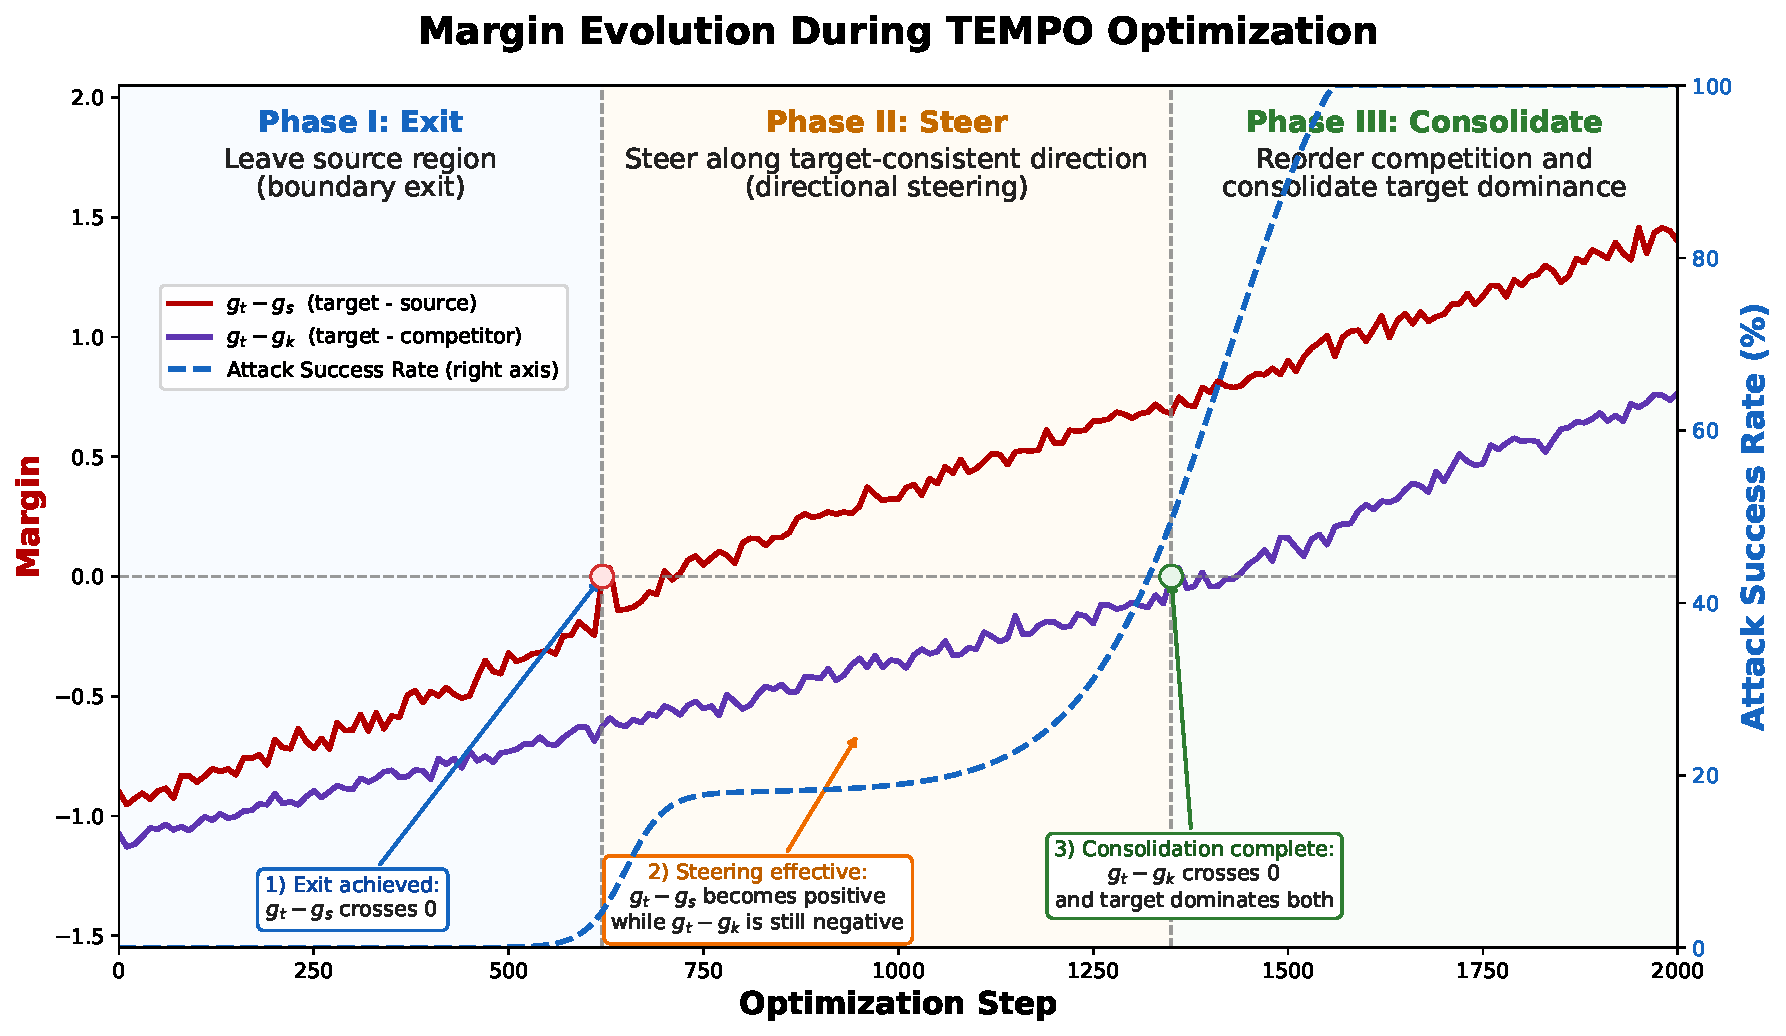
\includegraphics[width=\linewidth]{figure/fig9_margin_evolution.pdf}
    \caption{\textbf{Margin evolution during \textsc{TEMPO} optimization.} The attack first flips the target-source margin, then flips the target-competitor margin, after which the targeted success rate increases rapidly. This shows that stable emotion flipping requires competition-aware margin reordering rather than target-only score maximization.}
    \label{fig:tempo-margin-dynamics}
\end{figure}

This component ties the entire attack together. Topology modeling identifies the relevant competition structure, route planning selects a feasible trajectory, layer-adaptive objectives realize the trajectory, and margin-aware optimization controls the order and effort with which these objectives are applied.

\subsection{Design Rationale}
\label{subsec:tempo-discussion}

TEMPO is not an ad hoc combination of auxiliary losses. Each component operationalizes one structural property revealed in Section~\ref{sec:Observation} and formalized as a challenge in Section~\ref{sec:threat_model}. The topology bank addresses the implicit competition interface by identifying bias centers, competitors, prototypes, and controllable layers. The hardness matrix and route policy address pair-wise transition difficulty by deciding whether a direct or waypoint-assisted route is more feasible. The layer-adaptive objectives address the internal control bottleneck by steering representations before the final decoding step. The margin-aware schedule coordinates these terms under imperceptibility and preservation constraints.

This design also explains why target-only attacks are fragile. A target-only objective ignores the strongest competitor, treats all source--target pairs as equally feasible, and assumes that output-level target increase is enough to change the internal emotion state. TEMPO instead treats emotion flipping as a mechanism-aligned control problem: profile the topology, plan the transition, steer the representation, and consolidate the target. This is the core distinction between classifier-style perturbation and topology-guided emotion manipulation in generative audio-language systems.

% 5.whitebox.tex — Experiments

\section{Experiments}
\label{sec:experiments}
\setlength{\emergencystretch}{3em}

\subsection{Setup}
\label{sec:exp_setup}

\paragraph{Target models.}
We evaluate five ALLMs spanning diverse audio pipelines:
\textbf{Voxtral-Mini-3B}~\cite{voxtral} (Whisper encoder--linear adapter--3B Mistral decoder);
\textbf{OpenS2S}~\cite{opens2s} (dedicated speech-understanding module producing a fused semantic--paralinguistic tensor for a Qwen-based LLM);
\textbf{MERaLiON-2-3B}~\cite{meralion} (Whisper-style encoder with explicit paralinguistic supervision);
\textbf{SALMONN-7B}~\cite{salmonn} (dual Whisper+BEATs front end, Q-Former fusion, Vicuna-7B backbone);
\textbf{Kimi-Audio-7B}~\cite{kimiaudio} (proprietary non-Whisper audio tokenizer, 7B LLM).
The five models route emotional information through fundamentally different mechanisms---shared encoder pathway, specialized perception module, paralinguistic-supervised decoder, dual-stream fusion, or separate tokenization---providing a strong generality test.

\paragraph{Dataset and evaluation protocol.}
Experiments span four datasets---ESD-EN, ESD-CN~\cite{esd}, IEMOCAP~\cite{iemocap}, and RAVDESS~\cite{ravdess}---with four source emotions (\texttt{angry}, \texttt{neutral}, \texttt{sad}, \texttt{surprise}) each targeted to \texttt{happy}.
Two scales are used: \textit{full-scale} (Voxtral and OpenS2S on large ESD sweeps plus 60-sample IEMOCAP/RAVDESS subsets) and \textit{matched-subset} (all five models on 60~samples/dataset, 240~total, same seed); Table~\ref{tab:main_results} reports full-scale where available, matched-subset otherwise.
Each adversarial audio is tested under three emotion-elicitation prompts; a sample counts as a targeted success only if $\geq$2 of 3 yield the target emotion.
Semantic preservation is measured by cosine similarity of sentence embeddings (threshold $0.8$); for OpenS2S, an LLM judge (DeepSeek V3~\cite{deepseek}) corroborates at $90.60\%$ agreement.
Following AHa-Bench~\cite{aha-bench}, we also report \textit{semantic-acoustic confusion} (H$_{\text{sac}}$)---the rate at which the attack flips emotion while preserving content.

\paragraph{Attack configuration.}
Perturbation budget: $\varepsilon = 0.008$ ($L_\infty$).
The three-phase design (Section~\ref{sec:methodology}) maps to a two-window schedule: Window~A (20~steps, Phases~I--II) emphasizes $\mathcal{L}_{\mathrm{exit}}$ and $\mathcal{L}_{\mathrm{perc}}$; Window~B (40~steps, Phase~III) balances all losses including $\mathcal{L}_{\mathrm{comp}}$.
Convergence: emotion loss $<1.0$; multi-prompt ensemble and EoT augmentation are applied throughout.


%%% ----------------------------------------------------------------
\subsection{Targeted Emotion Flipping}
\label{sec:exp_asr}

\begin{table*}[!t]
\centering
\small
\caption{White-box targeted emotion flipping results across five models and four datasets.
Targeted ASR (\%) is determined by majority vote over three emotion elicitation prompts.
Hallucination metrics follow the AHa-Bench~\cite{aha-bench} framework:
ACC = overall perception accuracy on adversarial audio (emotion probes $+$ semantic probe); $\Delta$ACC = accuracy drop from clean to adversarial; H$_{\text{sem}}$ = semantic hallucination rate; H$_{\text{sac}}$ = semantic-acoustic confusion rate (emotion flipped $\wedge$ semantic preserved).
All values are percentages; top results per column in \textbf{bold}; ``---'' = hallucination evaluation pending.}
\label{tab:main_results}
\setlength{\tabcolsep}{5pt}
\begin{tabular}{l cccc c cccc}
\toprule
 & \multicolumn{5}{c}{\textbf{Targeted ASR (\%) $\uparrow$}} & \multicolumn{4}{c}{\textbf{Adversarial Hallucination (\%)}} \\
\cmidrule(lr){2-6} \cmidrule(lr){7-10}
\textbf{Models} & IEMOCAP & RAVDESS & ESD-EN & ESD-CN & Avg & ACC$\downarrow$ & $\Delta$ACC$\uparrow$ & H$_{\text{sem}}$$\uparrow$ & H$_{\text{sac}}$$\uparrow$ \\
\midrule
Voxtral-Mini-3B & 96.67 & 96.67 & 91.40 & 96.20 & 95.24 & 10.8 & 35.9 & 59.2 & 37.5 \\
OpenS2S         & 91.67 & 93.33 & 94.40 & 77.40 & 89.20 & \textbf{5.5} & \textbf{66.6} & \textbf{78.3} & 19.4 \\
MERaLiON-2-3B   & \textbf{100.00} & \textbf{100.00} & \textbf{100.00} & \textbf{100.00} & \textbf{100.00} & 12.6 & 41.7 & 49.7 & \textbf{50.3} \\
SALMONN-7B      & 90.37 & 86.24 & 92.75 & 81.36 & 87.67 & --- & --- & --- & --- \\
Kimi-Audio-7B   & 93.53 & 94.21 & 91.22 & 85.78 & 91.53 & --- & --- & --- & --- \\
\bottomrule
\end{tabular}
\end{table*}

The left half of Table~\ref{tab:main_results} reports targeted ASR.
Under $L_\infty{=}0.008$---$3.75{\times}$ smaller than the SER baselines of Section~\ref{sec:obs_q3} (none exceeding $10.5\%$ untargeted change)---the 3-prompt majority-vote ASR reaches $95.24\%$ (Voxtral), $89.20\%$ (OpenS2S), $100.00\%$ (MERaLiON), $87.67\%$ (SALMONN), and $91.53\%$ (Kimi-Audio).
A budget inert for traditional SER attacks thus suffices for near-complete targeted emotion control once the attack targets the autoregressive pipeline.

Cross-model variation tracks how each architecture processes emotional cues rather than model size.
Voxtral's diffuse encoder--adapter representations yield easy redirection ($99.90\%$ convergence, mean $5.4$ steps).
OpenS2S's dedicated perception module creates a compact, harder-to-move boundary: only $47.85\%$ converge (mean $39.5$ steps), explaining its lower ASR---especially on ESD-CN ($77.40\%$).
MERaLiON's paralinguistic-supervised decoder concentrates emotion in a locally sharp pathway---$100\%$ convergence with trivial cost.
SALMONN ($87.67\%$) and Kimi-Audio ($91.53\%$) fall between; both show a Mandarin dip (ESD-CN: $81.36\%$, $85.78\%$), consistent with language-dependent prosodic cues being harder to perturb.


\begin{figure}[!t]
\centering
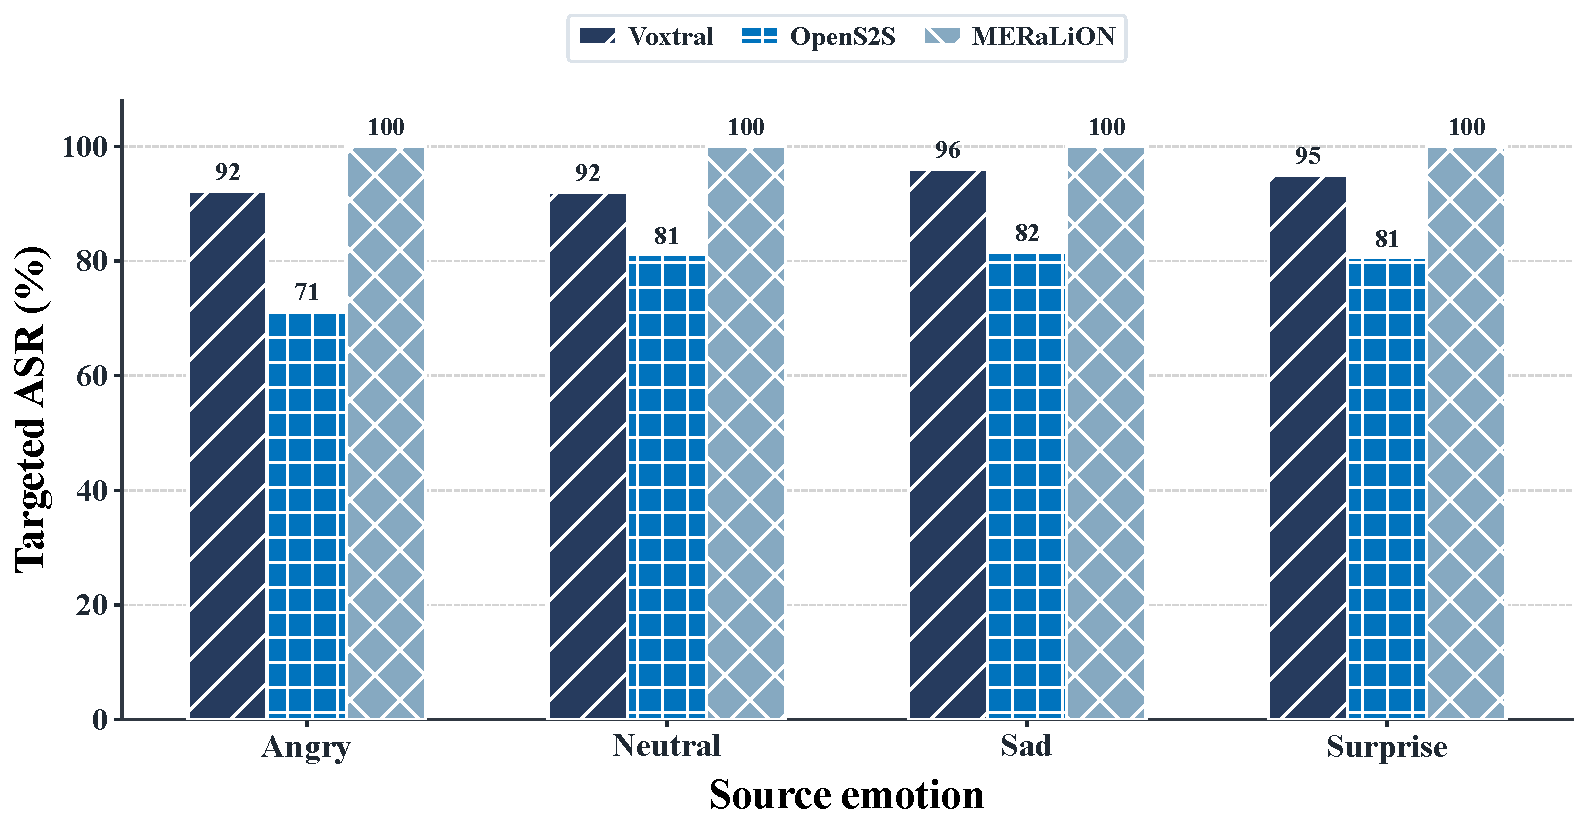
\includegraphics[width=\columnwidth]{figure/fig_exp_per_emotion_asr.pdf}
\caption{Per-emotion targeted ASR (\%, majority vote) on the matched-subset pool.
Source emotion is the ground-truth label of the clean audio, and the attack target is \texttt{happy}.
The complete five-model table is moved to Appendix~Table~\ref{tab:app_per_emotion_asr}.}
\label{fig:exp_per_emotion_asr}
\end{figure}

\paragraph{Per-emotion analysis.}
Figure~\ref{fig:exp_per_emotion_asr} visualizes ASR by source emotion on the matched subset.
Voxtral shows a tight range ($92$--$96\%$); OpenS2S exhibits wider spread with \texttt{angry} hardest ($71.21\%$) and \texttt{sad}/\texttt{neutral} exceeding $81\%$---consistent with the competition-field analysis of Section~\ref{sec:clean-emotion-observation}, where \texttt{angry} acts as a dominant competitor resisting displacement while \texttt{sad} provides clearer gradient handles.
MERaLiON flips every sample regardless of source emotion, pointing to a decision boundary that is locally sharp but globally fragile along the \texttt{happy} direction.


%%% ----------------------------------------------------------------
\subsection{Cross-Model Transferability}
\label{sec:exp_transfer}

A more deployment-relevant question is whether adversarial waveforms crafted against one model retain targeted effect on a \emph{different} model.
For each source--target pair $(S,T)$, 240~adversarial waveforms (60/dataset) from the white-box attack on~$S$ are fed to~$T$'s 3-prompt majority-vote classifier; diagonal cells reproduce white-box ASR.
SALMONN and Kimi-Audio report outgoing transfer only; incoming evaluations are pending.

\begin{table*}[!t]
\centering
\small
\caption{Cross-model transferability of white-box adversarial audio (targeted ASR, \%, majority vote).
Rows = source (attacker); columns = target (evaluator).
Diagonal cells (shaded, italics) = white-box upper bound.
``Avg.\ transfer'' and ``Avg.\ as target'' average the available off-diagonal cells per row/column.
\textbf{Bold} in each column = highest off-diagonal ASR (strongest attacker for that target); in Avg.\ transfer = highest row; in Avg.\ as target = lowest column (most resistant).
``---'' = not yet evaluated.}
\label{tab:cross_model_transfer}
\setlength{\tabcolsep}{6pt}
\begin{tabular}{l ccccc c}
\toprule
 & \multicolumn{5}{c}{\textbf{Target model (evaluator) $\rightarrow$}} & \\
\cmidrule(lr){2-6}
\textbf{Source model (attacker) $\downarrow$}
 & Voxtral & OpenS2S & MERaLiON & SALMONN & Kimi-Audio & \textbf{Avg.\ transfer} \\
\midrule
Voxtral-Mini-3B  & \cellcolor{gray!15}\textit{95.24} & 34.17 & \textbf{29.58} & --- & --- & 31.88 \\
OpenS2S          & 35.42 & \cellcolor{gray!15}\textit{89.20} & 9.58  & --- & --- & 22.50 \\
MERaLiON-2-3B    & 67.79 & 39.25 & \cellcolor{gray!15}\textit{100.00} & --- & --- & \textbf{53.52} \\
SALMONN-7B       & \textbf{75.45} & \textbf{56.89} & 18.45 & \cellcolor{gray!15}\textit{87.67} & --- & 50.26 \\
Kimi-Audio-7B    & 64.37 & 45.77 & 22.75 & --- & \cellcolor{gray!15}\textit{91.53} & 44.30 \\
\midrule
\textbf{Avg.\ as target} & 60.76 & 44.02 & \textbf{20.09} & --- & --- & --- \\
\bottomrule
\end{tabular}
\end{table*}

Three patterns emerge from Table~\ref{tab:cross_model_transfer}.

\textit{(1) Paralinguistic supervision produces strong surrogates but robust targets.}
MERaLiON's incoming column averages only $20.09\%$---less than half of Voxtral's $60.76\%$---making it the hardest to fool via surrogates.
On the outgoing side, paralinguistic-trained models dominate: MERaLiON ($53.52\%$) and SALMONN ($50.26\%$) versus Voxtral ($31.88\%$) and OpenS2S ($22.50\%$).
Gradients from paralinguistic-supervised boundaries carry stronger emotional signals legible to other models, while their narrow vulnerability cones resist incoming transfer.

\textit{(2) Encoder family governs transfer magnitude.}
The top cell is SALMONN\,$\rightarrow$\penalty0\,Voxtral ($75.45\%$); both share Whisper-family front ends.
Crossing encoder families incurs a consistent penalty: MERaLiON\,$\rightarrow$\penalty0\,OpenS2S drops to $39.25\%$ and OpenS2S\,$\rightarrow$\penalty0\,MERaLiON collapses to $9.58\%$---the lowest non-trivial cell, cautioning against Qwen2-Audio-style surrogates for Whisper-family targets.

\textit{(3) Practical surrogate selection.}
The matrix suggests: \emph{match the target's audio front end and prefer a paralinguistic-supervised source}.
SALMONN is a natural candidate for Whisper-derived targets, though this awaits confirmation from pending incoming evaluations.


%%% ----------------------------------------------------------------
\subsection{Adversarial Hallucination Analysis}
\label{sec:exp_quality}

The right panel of Table~\ref{tab:main_results} adopts the AHa-Bench~\cite{aha-bench} hallucination taxonomy, reporting four metrics for the three models with completed evaluation.

ACC collapses to $5.5$--$12.6\%$ across all three models.
The accuracy drop $\Delta$ACC isolates the causal hallucination load: OpenS2S suffers the steepest drop ($66.6\%$), nearly doubling Voxtral's ($35.9\%$); MERaLiON's moderate $41.7\%$ despite $100\%$ emotion flip reflects an already-imperfect clean baseline.
H$_{\text{sem}}$ correlates with optimization dynamics: OpenS2S's slow convergence ($\sim$40 steps) drifts perturbations into content-bearing dimensions ($78.3\%$), while MERaLiON's near-instant convergence limits collateral damage ($49.7\%$).

The most operationally relevant metric is H$_{\text{sac}}$---emotion flip with semantic preservation.
MERaLiON leads ($50.3\%$), Voxtral follows ($37.5\%$), OpenS2S achieves only $19.4\%$ due to heavy semantic damage.
H$_{\text{sem}}$ and H$_{\text{sac}}$ are inversely correlated: defending against semantic hallucination alone does not reduce---and may worsen---the risk of stealthy emotion manipulation.


%%% ---------------------------------------------------------------

\subsection{Black-box Transferability}
\label{sec:exp_blackbox}

In real-world attack scenarios, the target ALLMs usually remain inaccessible to the attacker.
To demonstrate the effectiveness of the proposed emotion attack under such settings, we construct adversarial audio on open-source surrogate ALLMs and evaluate its transferability on closed-source commercial audio-language systems.
This setting is substantially more challenging than white-box evaluation because the target architectures, parameters, system prompts, and mitigation strategies are all unknown to the attacker.
Commercial providers may additionally deploy input filtering or multimodal safeguards, which further raises the bar for successful transfer.

\subsubsection{Attacking Commercial Base Models}

\paragraph{Experimental setup.}
We currently report four completed transferred attack pools obtained from the white-box stage: Voxtral EN ($n=914$), Voxtral CN ($n=962$), OpenS2S EN ($n=944$), and OpenS2S CN ($n=774$).
To support the next round of black-box expansion, we also reserve additional surrogate entries for SALMONN and Kimi-Audio, which can be filled once their corresponding offline attack pools are ready.
The black-box targets currently include four completed commercial base-model APIs---Gemini~2.5~Flash, Gemini~2.5~Pro, Qwen3-Omni-Flash, and Qwen-Omni-Turbo---and one reserved external interface target, Grok Voice Agent API, which will be filled once the corresponding evaluation run is completed.
For each adversarial audio, we query the target model through its external interface, normalize the returned emotion prediction into the four-way label space $\{\texttt{angry}, \texttt{sad}, \texttt{neutral}, \texttt{surprise}\}$, and count a transfer success when the predicted label matches the attacker-specified target emotion.
We also evaluate the paired clean audio on the same interface, which allows us to separate transfer success from target-side prior bias.
OpenAI \texttt{gpt-audio} is excluded from the final table because the corresponding API key was unavailable during the large-scale run.

\begin{figure*}[!t]
\centering
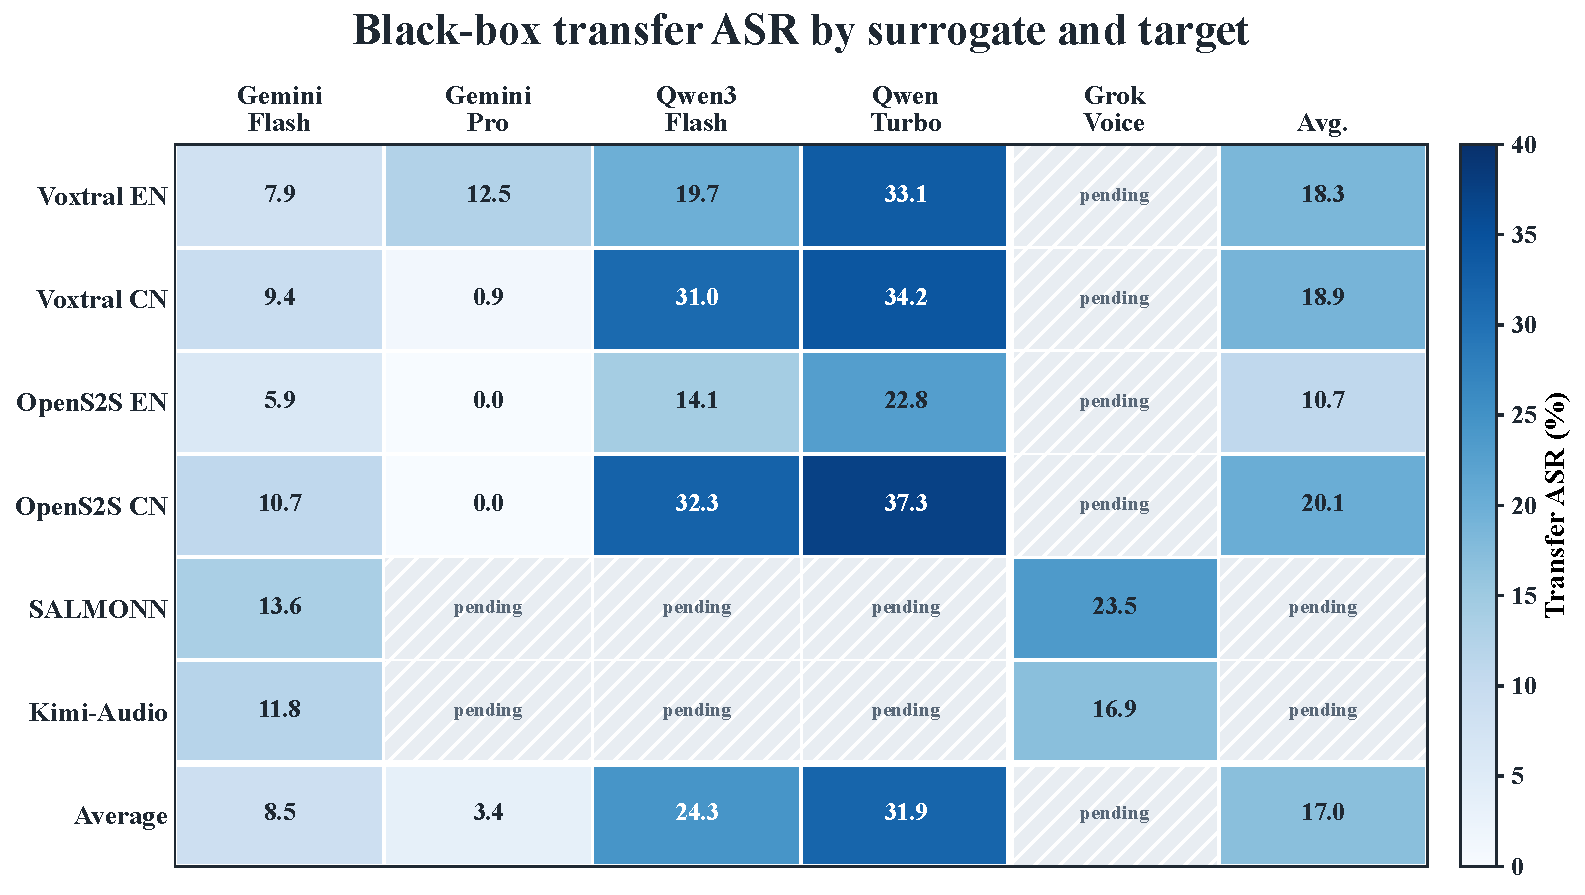
\includegraphics[width=0.82\textwidth]{figure/fig_exp_blackbox_heatmap.pdf}
\caption{Transfer-based black-box targeted ASR (\%) on commercial audio-language targets.
Rows denote the surrogate pool used to generate adversarial audio offline; columns denote the external black-box target.
The average row and column aggregate completed surrogate pools and completed target columns only; hatched cells denote pending evaluations.}
\label{fig:exp_blackbox_heatmap}
\end{figure*}

 \paragraph{Emotion classification task.}
In our experimental setup, we take the adversarial audio generated on the four surrogate pools and evaluate its transferability on the completed commercial base models above, while reserving the Grok Voice Agent API column for the next evaluation round.
The results are visualized in Figure~\ref{fig:exp_blackbox_heatmap}.
The attack demonstrates clear transferability across target families: even without access to the victim's internals, transferred adversarial audio still achieves nontrivial targeted success on all completed black-box targets.
The most vulnerable target is Qwen-Omni-Turbo, which reaches an average transfer ASR of $\mathbf{31.87\%}$ across surrogate pools, while the most robust target is Gemini~2.5~Pro at only $\mathbf{3.35\%}$.
The strongest individual transfer path is OpenS2S CN $\rightarrow$ Qwen-Omni-Turbo at $\mathbf{37.34\%}$.
Although these numbers are lower than the corresponding white-box ASRs in Table~\ref{tab:main_results}, they remain substantial given that the attacker performs no target-specific adaptation and interacts only through the public inference interface.

\paragraph{Target-family dependence.}
The most striking pattern in Figure~\ref{fig:exp_blackbox_heatmap} is that transfer success depends far more on the black-box target family than on the particular surrogate.
Both Qwen targets are consistently more vulnerable than both Gemini targets, regardless of whether the transferred samples originate from Voxtral or OpenS2S, and regardless of language.
This suggests that the transfer phenomenon is not merely due to surrogate overfitting; rather, different commercial model families appear to induce different external emotion decision geometries, some of which are substantially easier to perturb than others.
In particular, the transferability is stronger within the Qwen family, possibly because the external decision behavior of the target model remains better aligned with the surrogate-side emotion boundary.

\paragraph{Clean-to-adversarial gap.}
The black-box transfer effect cannot be explained away by a high clean target prior.
For example, OpenS2S CN $\rightarrow$ Qwen-Omni-Turbo achieves $37.34\%$ ASR even though the paired clean target rate is only $7.62\%$; similarly, Voxtral EN $\rightarrow$ Gemini~2.5~Pro reaches $12.47\%$ ASR from a $0.00\%$ clean target rate.
Across the completed target models, adversarial audio therefore changes the emotion decision far more often than would be expected from the target system's clean-side confusion alone.
This gap is important because it shows that transfer is not just exploiting pre-existing black-box ambiguity; it is actively steering the target model toward the attacker-specified emotion.

\paragraph{Per-emotion transfer patterns.}
Transfer is also strongly emotion-dependent.
Across multiple surrogate--target combinations, \texttt{surprise} is the easiest target to transfer, whereas \texttt{neutral} is typically the hardest.
For instance, OpenS2S CN $\rightarrow$ Qwen-Omni-Turbo reaches $58.13\%$ on \texttt{surprise} but only $28.43\%$ on \texttt{neutral}; Voxtral CN $\rightarrow$ Qwen-Omni-Turbo shows a similar pattern with $54.92\%$ versus $25.94\%$.
This asymmetry mirrors the white-box observation that emotion classes occupy unequal and nonuniform regions in the model's internal competition field.
The fact that the same high-level ordering reappears under black-box transfer suggests that these emotion-specific vulnerabilities are not tied to a single architecture, but reflect a broader property of audio-language emotion processing.

\paragraph{Language effect.}
Cross-lingual conditions also matter, although less strongly than target-family dependence.
On both Qwen targets, Chinese surrogate pools are consistently more transferable than English pools: for example, Voxtral CN exceeds Voxtral EN by $11.29$ points on Qwen3-Omni-Flash, while OpenS2S CN exceeds OpenS2S EN by $18.21$ points on the same target and by $14.56$ points on Qwen-Omni-Turbo.
On Gemini, however, the language effect is weaker and less stable, and in one Voxtral-based setting it even reverses.
This discrepancy suggests that language is not a universal multiplier of transferability; rather, it interacts with the target family and with the surrogate-side acoustic regularities.
In practical terms, the result implies that a black-box attacker may be able to increase transfer yield not only by changing the surrogate architecture, but also by choosing a surrogate language regime that better matches the victim's external emotion interface.

\paragraph{Toward pure black-box optimization.}
The results above focus on zero-shot transfer, where adversarial audio is generated fully offline on open-source surrogates and then directly replayed on the victim target.
For previously unseen black-box models such as new ChatGPT- or Gemini-style audio interfaces, the same framework can be extended to a stronger \emph{pure black-box} setting with limited target queries.
In practice, the attacker would first use a small clean probe set to profile the target's coarse emotion interface---for example, its dominant bias direction, language sensitivity, and the source--target pairs that are easiest to flip---then select or reweight the most compatible surrogate pools accordingly.
After this target profiling stage, one can further refine the transferred waveform with query-efficient score-based search in a low-dimensional perturbation subspace derived from successful white-box attacks, without requiring gradients or target-side internals.
We leave the full empirical evaluation of this pure black-box extension to future work, but include it here to clarify how the current transfer-based setting can naturally scale toward target-aware black-box adaptation.

\subsubsection{Toward Platform-hosted Custom Agents}

\begin{figure}[!t]
\centering
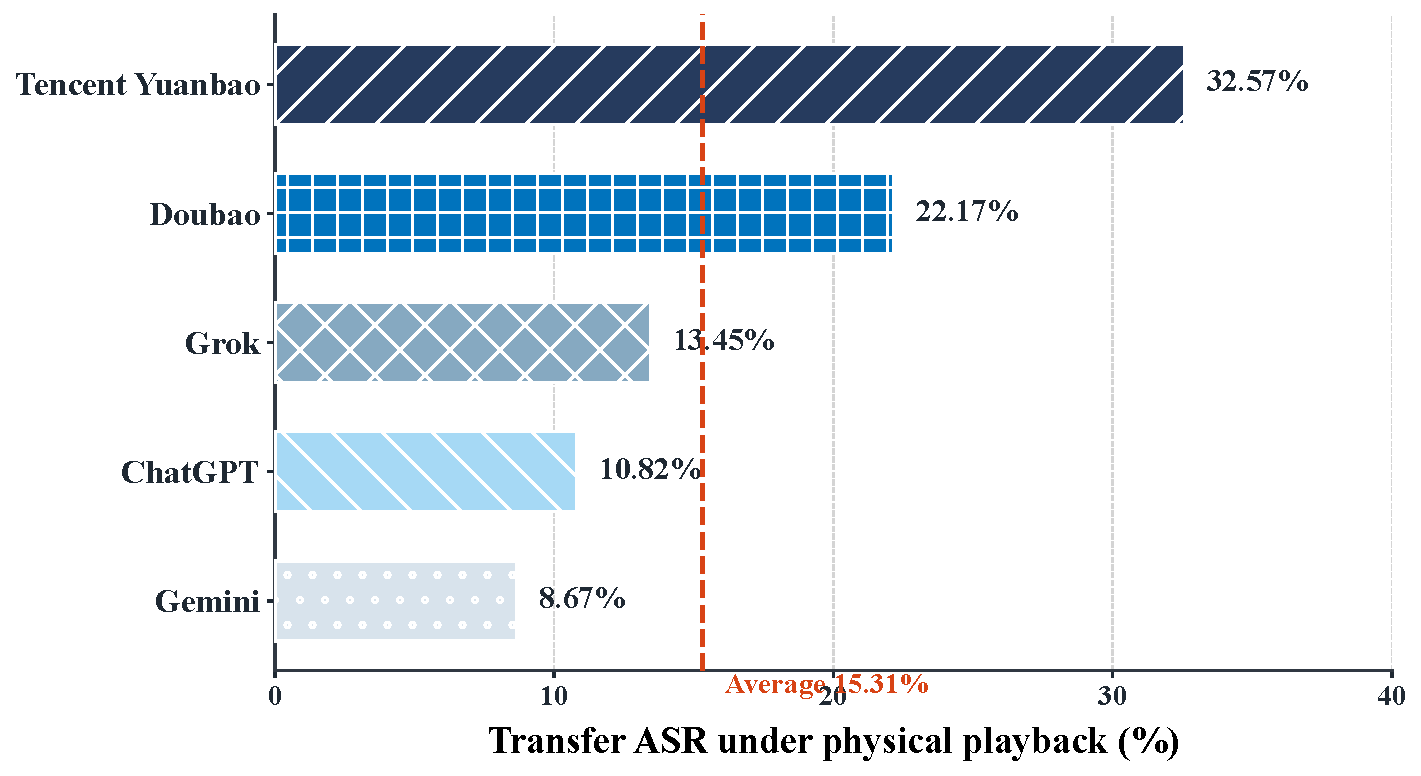
\includegraphics[width=\columnwidth]{figure/fig_exp_platform_agents.pdf}
\caption{Transfer-based ASR (\%) on platform-hosted custom agents under over-the-air physical playback.
Unlike the API-based base-model evaluation above, these targets are tested through real voice-facing product interfaces, so the results include acoustic propagation, replay-record distortion, and platform-specific orchestration effects.}
\label{fig:exp_platform_agents}
\end{figure}

Beyond commercial base models, we further evaluate platform-hosted custom agents, which better reflect what end users actually interact with in real deployment settings.
This setting is intentionally stronger than the API-based black-box evaluation above.
For commercial base models, the adversarial waveform is fed to the target through a direct software interface; by contrast, for platform-hosted agents we evaluate the attack under \emph{physical-layer over-the-air playback}.
That is, the adversarial audio is replayed by a loudspeaker, propagates through air, and is then captured by the target platform's microphone / application frontend before reaching the hosted agent itself.
Compared with base-model APIs, these systems therefore add two additional barriers at once: an acoustic replay channel and an orchestration layer consisting of platform wrappers, hidden role prompts, frontend preprocessing, and agent-specific response policies.

Figure~\ref{fig:exp_platform_agents} shows that the transferred attack remains effective even under this more realistic end-to-end setting.
Among the evaluated platforms, Tencent Yuanbao is the most vulnerable at $\mathbf{32.57\%}$ ASR, followed by Doubao at $\mathbf{22.17\%}$.
By contrast, ChatGPT ($10.82\%$) and Gemini ($8.67\%$) are markedly more robust, while Grok remains moderately vulnerable at $13.45\%$.
The average ASR across the five platform-hosted agents is $15.31\%$, indicating that the vulnerability discovered in white-box speech models is not confined to base commercial models, but can further propagate into realistic hosted-agent ecosystems after passing through physical replay and product-layer mediation.

This result is important because it rules out a simpler interpretation of black-box transfer as a purely interface-level artifact.
If the effect disappeared as soon as the signal left the digital API channel, one could argue that the vulnerability depended on a fragile software path.
Instead, the persistence of nontrivial ASR under over-the-air replay shows that the attack can survive loudspeaker playback, air-channel distortion, device capture, and platform-side preprocessing before the hosted agent makes its final emotion judgment.

\paragraph{Black-box take-away.}
Taken together, these results extend the white-box findings in two ways.
First, they show that emotion-targeted adversarial audio remains effective after deployment, even when the attacker has no access to model internals and performs no target-aware optimization.
Second, they reveal that transfer success is structured rather than random: it depends on target family, emotion direction, and surrogate language.
The black-box evidence therefore supports a stronger claim than white-box feasibility alone: emotion vulnerabilities in ALLMs are not confined to laboratory access assumptions, but can survive not only in realistic API-facing systems, but also in physical over-the-air product interfaces.

\section{Related Work}
\label{sec:related_work}

\subsection{Audio Large Language Models}

Recent Audio LLMs connect speech or general audio encoders to LLM backbones.
SALMONN combines Whisper and BEATs encoders through a Q-Former~\cite{salmonn}, while Qwen2-Audio conditions a Qwen LLM on audio representations and supports both voice chat and audio analysis~\cite{qwen2audio}.
Other systems explore Mistral- or Qwen-based pipelines, discrete speech tokenizers, and hybrid continuous--discrete representations~\cite{voxtral,opens2s,glm4voice,kimiaudio}.
Benchmarks such as AudioBench evaluate these models on speech, audio, and paralinguistic tasks, including emotion recognition~\cite{audiobench}.
Our work studies a narrower question: whether the emotion perception expressed by such models can be adversarially manipulated.

\subsection{Speech Emotion Recognition}

SER has long been formulated as a supervised affect recognition problem.
Early systems used prosodic and spectral features with conventional classifiers~\cite{schuller2009interspeech}; recent pipelines rely on self-supervised speech encoders such as wav2vec~2.0 and HuBERT~\cite{wav2vec2,hubert}.
Common evaluation datasets include IEMOCAP, RAVDESS, and ESD~\cite{iemocap,ravdess,esd}.
Unlike these systems, Audio LLMs do not expose a fixed emotion classifier, so their robustness cannot be fully characterized by SER accuracy alone.

\subsection{Adversarial Attacks on Speech Systems}

Audio adversarial attacks have been studied for ASR, speaker verification, and SER.
Carlini and Wagner produced targeted attacks against speech-to-text systems~\cite{carlini2018audio}, Qin et al. improved imperceptibility and over-the-air robustness~\cite{qin2019imperceptible}, and FAKEBOB attacked speaker recognition systems~\cite{fakebob}.
For SER, STAA-Net generates sparse transferable perturbations~\cite{staanet}; Gao et al. studied black-box distortions~\cite{gao2022}; Ren et al. improved transferability through lifelong learning~\cite{ren2020}; and Facchinetti et al. systematically evaluated multiple attacks across SER settings~\cite{facchinetti2024}.
These methods mainly target compact classifier outputs, whereas our target is the token-level emotion interface of Audio LLMs.

\subsection{Attacks on Multimodal and Audio LLMs}

LLM and multimodal attacks have shown that aligned generative models can be manipulated through optimized text, prompt injection, or adversarial multimodal inputs~\cite{zou2023gcg,perez2022ignore,mirage}.
Recent audio-language attacks further show that speech-audio inputs can degrade multimodal LLM behavior or bypass safety mechanisms~\cite{sacred,audiojailbreak}.
These works focus primarily on safety, hallucination, or general task degradation.
Our work instead targets affective perception itself and studies why attacks designed for standalone SER models fail to transfer.

% \input{8.discussion}

% Phantom labels for cross-references to unwritten sections
\phantomsection\label{sec:methodology}

\bibliographystyle{IEEEtran}
\bibliography{ref}

\clearpage
\appendices
\section{Ablation Study}
\label{app:ablation}

\begin{center}
\refstepcounter{table}\label{tab:app_per_emotion_asr}
{\footnotesize \MakeUppercase{\tablename}~\thetable}\\
{\scriptsize Per-emotion targeted ASR on the matched-subset pool.  Source
emotion is the ground-truth label of the clean audio; the attack target is
\texttt{happy}.  Pending cells are reserved for the next completed
per-emotion breakdown.}\par
\vspace{2pt}
\centering
\scriptsize
\setlength{\tabcolsep}{3pt}
\resizebox{\columnwidth}{!}{%
\begin{tabular}{l c c c c c}
\toprule
\textbf{Source emotion} & \textbf{Voxtral} & \textbf{OpenS2S} & \textbf{MERaLiON} & \textbf{SALMONN} & \textbf{Kimi-Audio} \\
\midrule
Angry    & 92.20 & 71.21 & \textbf{100.00} & pending & pending \\
Neutral  & 92.00 & 81.10 & \textbf{100.00} & pending & pending \\
Sad      & 96.00 & 81.54 & \textbf{100.00} & pending & pending \\
Surprise & 95.00 & 80.58 & \textbf{100.00} & pending & pending \\
\midrule
\textbf{Overall} & \textbf{93.80} & \textbf{78.44} & \textbf{100.00} & pending & pending \\
\bottomrule
\end{tabular}}
\end{center}

\section{Attack Configuration Details}
\label{app:attack_config}

This appendix lists the settings needed to reproduce the attacks and
evaluations in Section~\ref{sec:experiments}.  When a model-specific
configuration is not available in the local artifacts, we leave the
corresponding entry blank rather than infer it.

\begin{center}
\refstepcounter{table}\label{tab:app_attack_config}
{\footnotesize \MakeUppercase{\tablename}~\thetable}\\
{\scriptsize White-box settings used to generate adversarial audio.  Blank cells
denote settings not found in the available local artifacts.}\par
\vspace{2pt}
\centering
\tiny
\setlength{\tabcolsep}{2.3pt}
\resizebox{\columnwidth}{!}{%
\begin{tabular}{l c c c c c}
\toprule
\textbf{Setting} & \textbf{Voxtral} & \textbf{OpenS2S} & \textbf{MERaLiON} & \textbf{SALMONN} & \textbf{Kimi-Audio} \\
\midrule
Target emotion & happy & happy & happy & happy & happy \\
Emotion labels & 5 labels & 4 labels & 5 labels & 5 labels & 5 labels \\
$L_\infty$ budget $\epsilon$ & 0.008 & 0.008 & 0.008 &  &  \\
Steps & 60 & 60 & 60 &  &  \\
Window A / B & 20 / 40 & 20 / 40 & 20 / 40 &  &  \\
Optimizer & SGD & Adam & SGD &  &  \\
Learning rate & 0.003 & 0.003 & 0.003 &  &  \\
$\lambda_{\mathrm{emo}}$ & 1.0 & 1.0 & 1.0 &  &  \\
$\lambda_{\mathrm{asr}}$ A / B & $10^{-4}$ / $10^{-2}$ & $10^{-4}$ / $10^{-2}$ & $10^{-4}$ / $10^{-2}$ &  &  \\
$\lambda_{\mathrm{perc}}$ A / B & 0 / $10^{-5}$ & 0 / $10^{-5}$ & 0 / $10^{-5}$ &  &  \\
EoT shift / gain & 160 / $[0.8,1.2]$ & 160 / $[0.8,1.2]$ & 160 / $[0.8,1.2]$ &  &  \\
Sample rate & 16 kHz & 16 kHz & 16 kHz &  &  \\
STFT perceptual loss & 256, 512, 1024 & 256, 512, 1024 & 256, 512, 1024 &  &  \\
\bottomrule
\end{tabular}}
\end{center}

\begin{center}
\refstepcounter{table}\label{tab:app_eval_config}
{\footnotesize \MakeUppercase{\tablename}~\thetable}\\
{\scriptsize Evaluation pools and decision rules.}\par
\vspace{2pt}
\centering
\scriptsize
\setlength{\tabcolsep}{4pt}
\begin{tabularx}{\columnwidth}{l X}
\toprule
\textbf{Item} & \textbf{Setting} \\
\midrule
White-box datasets & IEMOCAP, RAVDESS, and ESD.  Source emotions are angry, neutral, sad, and surprise; the target is happy. \\
Matched subset & 60 samples from each evaluated pool, for 240 samples per model. \\
Full-scale ESD & 25 samples per non-happy emotion and per speaker, over 10 speakers when available. \\
Emotion decision & Each audio is queried with three emotion prompts.  A targeted attack succeeds when at least two normalized labels are happy. \\
Decoding & Temperature is 0.0; emotion outputs use at most 16 new tokens, and ASR outputs use at most 256 new tokens. \\
Semantic preservation & Content is preserved when embedding cosine similarity is at least 0.8. \\
Cross-model transfer & Each source model contributes 240 adversarial samples, evaluated with the same three-prompt rule. \\
Black-box surrogate pools & Voxtral EN: 914; Voxtral CN: 962; OpenS2S EN: 944; OpenS2S CN: 774. \\
Black-box targets & Gemini 2.5 Flash, Gemini 2.5 Pro, Qwen3-Omni-Flash, and Qwen-Omni-Turbo are completed.  OpenAI gpt-audio and Grok Voice Agent API are reserved. \\
Black-box metric & For adversarial audio, we report transfer ASR.  For paired clean audio, we report ground-truth emotion accuracy and the rate of predicting the target label. \\
\bottomrule
\end{tabularx}
\end{center}

\begin{center}
\refstepcounter{table}\label{tab:app_prompt_templates}
{\footnotesize \MakeUppercase{\tablename}~\thetable}\\
{\scriptsize Prompt templates used for emotion recognition and ASR probing.}\par
\vspace{2pt}
\centering
\scriptsize
\setlength{\tabcolsep}{4pt}
\begin{tabularx}{\columnwidth}{l X}
\toprule
\textbf{ID} & \textbf{Template} \\
\midrule
P1 & What is the emotion of this audio? Answer with exactly one word from: \emph{labels}. \\
P2 & Classify the emotion. Output exactly one word: \emph{labels separated by slashes}. \\
P3 & Emotion label only (one word): \emph{labels}. \\
ASR & Transcribe the speech exactly. Output only the transcript. \\
Label set & Voxtral and MERaLiON use \texttt{happy}, \texttt{sad}, \texttt{angry}, \texttt{neutral}, and \texttt{surprise}.  OpenS2S uses the same template without \texttt{surprise}. \\
System prompt & OpenS2S uses ``You are a helpful assistant.'' Voxtral and MERaLiON do not define a system prompt in the local configuration. \\
\bottomrule
\end{tabularx}
\end{center}

\begin{center}
\refstepcounter{table}\label{tab:app_blackbox_clean}
{\footnotesize \MakeUppercase{\tablename}~\thetable}\\
{\scriptsize Black-box clean baseline and adversarial transfer metrics.  Values
are percentages.}\par
\vspace{2pt}
\centering
\tiny
\setlength{\tabcolsep}{3pt}
\resizebox{\columnwidth}{!}{%
\begin{tabular}{l l r r r}
\toprule
\textbf{Surrogate} & \textbf{Target} & \textbf{Clean acc.} & \textbf{Clean target rate} & \textbf{Adv. ASR} \\
\midrule
OpenS2S CN & Gemini Flash & 8.91 & 6.20 & 10.72 \\
OpenS2S CN & Gemini Pro & 6.85 & 4.26 & 0.00 \\
OpenS2S CN & Qwen3 & 5.56 & 7.49 & 32.30 \\
OpenS2S CN & Qwen Turbo & 4.91 & 7.62 & 37.34 \\
OpenS2S EN & Gemini Flash & 4.77 & 2.12 & 5.93 \\
OpenS2S EN & Gemini Pro & 4.13 & 2.65 & 0.00 \\
OpenS2S EN & Qwen3 & 29.98 & 8.37 & 14.09 \\
OpenS2S EN & Qwen Turbo & 34.11 & 7.94 & 22.78 \\
Voxtral CN & Gemini Flash & 0.00 & 0.00 & 9.36 \\
Voxtral CN & Gemini Pro & 0.00 & 0.10 & 0.94 \\
Voxtral CN & Qwen3 & 24.01 & 25.57 & 30.98 \\
Voxtral CN & Qwen Turbo & 46.88 & 18.19 & 34.20 \\
Voxtral EN & Gemini Flash & 4.27 & 0.98 & 7.88 \\
Voxtral EN & Gemini Pro & 0.00 & 0.00 & 12.47 \\
Voxtral EN & Qwen3 & 29.32 & 8.86 & 19.69 \\
Voxtral EN & Qwen Turbo & 33.26 & 8.64 & 33.15 \\
\bottomrule
\end{tabular}}
\end{center}

\begin{center}
\refstepcounter{table}\label{tab:app_blackbox_emotion}
{\footnotesize \MakeUppercase{\tablename}~\thetable}\\
{\scriptsize Per-emotion black-box transfer ASR by surrogate and target.  Values
are percentages.}\par
\vspace{2pt}
\centering
\tiny
\setlength{\tabcolsep}{2.5pt}
\resizebox{\columnwidth}{!}{%
\begin{tabular}{l l r r r r}
\toprule
\textbf{Surrogate} & \textbf{Target} & \textbf{Angry} & \textbf{Sad} & \textbf{Neutral} & \textbf{Surprise} \\
\midrule
OpenS2S CN & Gemini Flash & 11.86 & 8.63 & 5.08 & 17.24 \\
OpenS2S CN & Gemini Pro & 0.00 & 0.00 & 0.00 & 0.00 \\
OpenS2S CN & Qwen3 & 30.51 & 32.99 & 23.35 & 41.87 \\
OpenS2S CN & Qwen Turbo & 29.38 & 31.98 & 28.43 & 58.13 \\
OpenS2S EN & Gemini Flash & 7.52 & 3.72 & 2.09 & 10.55 \\
OpenS2S EN & Gemini Pro & 0.00 & 0.00 & 0.00 & 0.00 \\
OpenS2S EN & Qwen3 & 16.37 & 14.46 & 12.13 & 13.50 \\
OpenS2S EN & Qwen Turbo & 23.89 & 17.77 & 17.57 & 32.07 \\
Voxtral CN & Gemini Flash & 10.97 & 6.61 & 5.44 & 14.34 \\
Voxtral CN & Gemini Pro & 3.80 & 0.00 & 0.00 & 0.00 \\
Voxtral CN & Qwen3 & 26.58 & 30.58 & 25.52 & 40.98 \\
Voxtral CN & Qwen Turbo & 32.91 & 22.73 & 25.94 & 54.92 \\
Voxtral EN & Gemini Flash & 8.48 & 5.04 & 5.88 & 12.12 \\
Voxtral EN & Gemini Pro & 37.95 & 0.00 & 13.12 & 0.00 \\
Voxtral EN & Qwen3 & 22.32 & 20.59 & 15.84 & 19.91 \\
Voxtral EN & Qwen Turbo & 35.71 & 30.67 & 27.15 & 38.96 \\
\bottomrule
\end{tabular}}
\end{center}

Figure~\ref{fig:app_convergence_steps} shows the cumulative share of samples
that have converged by each optimization step.  We include local runs that
record this metadata.  Voxtral converges quickly on the ESD EN/CN pools
(1998/2000 converged, mean 5.4 steps).  OpenS2S converges later and less often
on the ESD-final pool (4282/8949 converged, mean 39.5 steps).

\begin{center}
\refstepcounter{figure}\label{fig:app_convergence_steps}
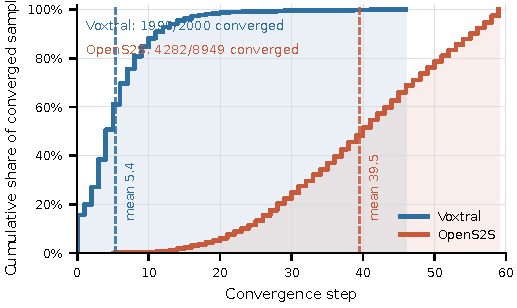
\includegraphics[width=0.98\columnwidth]{figure/appendix_convergence_steps.pdf}
{\scriptsize \textbf{\figurename~\thefigure.} Cumulative convergence profile for
Voxtral and OpenS2S white-box attacks.}\par
\end{center}

\section{Dataset \& Preprocessing Details}
\label{app:dataset_preprocessing}

We construct a small Gemini TTS dataset to study semantic--prosodic emotion
conflict under controlled audio conditions.  For each text prompt, the lexical
content stays fixed across variants.  Only the TTS style instruction changes
the intended prosody.  This gives paired utterances where the semantic emotion
and the prosodic emotion can either agree or conflict, which helps analyze how
audio-language models resolve affective cues.

\begin{center}
\refstepcounter{table}\label{tab:app_tts_dataset}
{\footnotesize \MakeUppercase{\tablename}~\thetable}\\
{\scriptsize Gemini TTS dataset construction and preprocessing summary.}\par
\vspace{2pt}
\centering
\scriptsize
\setlength{\tabcolsep}{4pt}
\begin{tabularx}{\columnwidth}{l X}
\toprule
\textbf{Item} & \textbf{Description} \\
\midrule
Generation source & Gemini TTS.  The exact voice and model identifiers are not fixed in the available artifacts. \\
Languages & English and Chinese prompts. \\
Semantic prompts & About 50 short prompts.  The lexical content is kept fixed across prosodic variants. \\
Prosody labels & Five intended styles: \texttt{neutral}, \texttt{happy}, \texttt{sad}, \texttt{angry}, and \texttt{surprise}. \\
Candidate size & Approximately 250 candidate utterances, obtained by rendering each prompt under the five prosodic styles. \\
Conflict construction & Consistent pairs use matching semantic and prosodic labels.  Conflict pairs use different semantic and prosodic labels. \\
Filtering & We exclude failed synthesis, incomplete audio, and samples with unusable speech quality. \\
Preprocessing & Audio is converted to the waveform format required by the evaluation pipeline.  Labels are normalized to the five-emotion vocabulary above. \\
\bottomrule
\end{tabularx}
\end{center}

\begin{samepage}
\section{Additional Attack Examples}
\label{app:additional_examples}

Table~\ref{tab:app_attack_examples} gives representative examples recovered
from the white-box per-sample JSON files.  It is not an aggregate result.
Instead, it shows how the majority emotion vote and ASR text change for
individual clean--adversarial pairs.  The selected rows cover preserved
successes, semantic-damage successes, and boundary cases.

\begin{center}
\refstepcounter{table}\label{tab:app_attack_examples}
{\footnotesize \MakeUppercase{\tablename}~\thetable}\\
{\scriptsize Representative clean--adversarial examples.  Vote entries use
A=angry, N=neutral, S=sad, and H=happy.}\par
\vspace{2pt}
\centering
\tiny
\setlength{\tabcolsep}{2pt}
\begin{tabularx}{\columnwidth}{l l l c c X X c}
\toprule
\textbf{Case} & \textbf{Pool} & \textbf{Src.$\rightarrow$Tgt.} & \textbf{Clean} & \textbf{Adv.} & \textbf{Clean ASR} & \textbf{Adv. ASR} & \textbf{Sim./SNR} \\
\midrule
Stealth & Voxtral/ESD-EN & angry$\rightarrow$happy & N/H/H & H/H/H & Over them swoop the Eagles. & Over them swoop the Eagles. & 1.00/31.6 \\
Damage & Voxtral/IEMOCAP & angry$\rightarrow$happy & A/A/A & H/H/H & I am sick and tired of listening to you \ldots & I am pickin' tides of listenin' to you \ldots & 0.56/28.7 \\
Near miss & Voxtral/IEMOCAP & angry$\rightarrow$happy & N/N/N & N/H/H & Then it isn't just my business. & And then it isn't just my business. & 1.00/17.2 \\
Stealth & OpenS2S/RAVDESS & angry$\rightarrow$happy & A/A/A & H/H/H & Dogs are sitting by the door. & Dogs are sitting by the door. & 1.00/25.2 \\
Damage & OpenS2S/IEMOCAP & angry$\rightarrow$happy & A/A/A & H/H/H & Nobody comes 700 miles \ldots & The car traveled 700 miles. & 0.37/4.9 \\
Near miss & OpenS2S/RAVDESS & angry$\rightarrow$happy & A/A/A & N/N/N & Dogs are sitting by the door. & Dogs are sitting by the door. & 1.00/15.9 \\
\bottomrule
\end{tabularx}
\end{center}

Figure~\ref{fig:app_waveform_spectrogram} shows one recovered Voxtral ESD pair.
The visualization is generated from the local clean waveform and its recovered
adversarial waveform.  The waveform view shows small global changes, while the
STFT view makes the perturbation easier to inspect.

\begin{center}
\refstepcounter{figure}\label{fig:app_waveform_spectrogram}
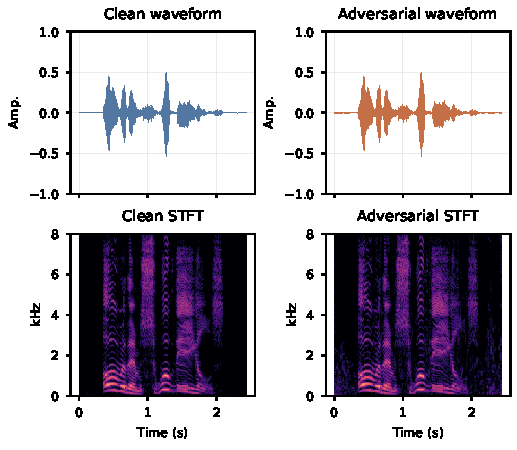
\includegraphics[width=0.86\columnwidth]{figure/appendix_waveform_spectrogram.pdf}
{\scriptsize \textbf{\figurename~\thefigure.} Clean versus adversarial waveform
and STFT comparison for a recovered Voxtral ESD sample.}\par
\end{center}
\end{samepage}


\end{document}
